%%%%%%%%%%%%%%%%%%%%%%%%%%%%%%%%%%%%%%%%%%%%%%%%%%%%%%%
% A template for Wiley article submissions.
% Developed by Overleaf. 
%
% Please note that whilst this template provides a 
% preview of the typeset manuscript for submission, it 
% will not necessarily be the final publication layout.
%
% Usage notes:
% The "blind" option will make anonymous all author, affiliation, correspondence and funding information.
% Use "num-refs" option for numerical citation and references style.
% Use "alpha-refs" option for author-year citation and references style.

\documentclass[alpha-refs]{wiley-article-02b}
% \documentclass[blind,num-refs]{wiley-article}

% Add additional packages here if required
\usepackage{siunitx}

% For figures
\usepackage{graphics}

%For captions - even though template has complex caption commands
\usepackage[labelfont=bf,justification=centering]{caption}
\usepackage[font=small,labelfont=bf]{subcaption}
\captionsetup[sub]{font=small,labelfont={bf,sf}}

%% For figures numbered by section
\usepackage{chngcntr}
\counterwithin{figure}{section}
\counterwithin{table}{section}

%% Additional links for hyperref
\usepackage[unicode=true,pdfusetitle,
bookmarks=true,bookmarksnumbered=true,bookmarksopen=true,bookmarksopenlevel=2,
 breaklinks=false,pdfborder={0 0 1},backref=false,colorlinks=false]
 {hyperref}
\hypersetup{pdfstartview={XYZ null null 1}}

\usepackage[backend=bibtex,
			natbib=true, 
			style=chicago-authordate]{biblatex}
\addbibresource{Returns.bib}


\usepackage{lipsum}

\usepackage{lmodern}
\newcommand{\graph}[3]{
\raisebox{-#1mm}{\includegraphics[height=#2em,width=3cm]{#3}}
}

\usepackage{booktabs} % for vertically partitioned table

%%%%%%%%#################################################################################%%%%%%%%%%%%%%%%%%%%%%%%%%%%%

% Update article type if known
\papertype{WORLD BANK EDUCATION GLOBAL PRACTICE}
% Include section in journal if known, otherwise delete
\paperfield{Russian Federation: Analytical Services and Advisory Activity: 
P170978}

\title{Returns to Education in the Russian Federation: Does depreciation explain some recent trends?}

% List acknowledgments here.
\fundinginfo{Thanks are due to the Higher School of Economics, Moscow for making the Russian Longitudinal Monitoring Study (RLMS) Household data readily available for reseachers around the world. Thanks are also due to Sylvain Weber for generously sharing the code from his University of Geneva Doctoral Thesis, which we adapted for one of the reported sets of estimations. The code used for this paper is made freely available for all researchers at \url{https://bitbucket.org/zagamog/edreru/src/master/}}

% Include full author names and degrees, when required by the journal.
% Use the \authfn to add symbols for additional footnotes and present addresses, if any. Usually start with 1 for notes about author contributions; then continuing with 2 etc if any author has a different present address.

\author[*]{Ekaterina Melianova}
\author[*]{\hspace{-1em}Suhas Parandekar}
\author[*]{\hspace{-1em}Art\"{e}m Volgin}

% List abbreviations here, if any. Please note that it is preferred that abbreviations be defined at the first instance they appear in the text, rather than creating an abbreviations list.
\acks{\begin{normalsize}
\emph{Country Director:} Renaud Seligman; \emph{Regional Director:} Fadia Saadah; \emph{Practice Manager:} Harry Patrinos; \emph{Program Leader:} Dorota Nowak; \emph{Peer Reviewers}: Cristian Aedo; Ruslan Yemtsov; Husein Abdul-Hamid; \emph{Team members:} Polina Zavalina; Zhanna Terlyga. Thanks to seminar participants at the World Bank Moscow office on Jan. 29, 2020 for useful feedback. Any errors are a responsibility of the authors.
\end{normalsize}
\vspace{-0.2in}}

%\contrib[\authfn{1}]{Equally contributing authors.}

% Include full affiliation details for all authors
\affil[*]{Education Global Practice, Europe and Central Asia}

%\corraddress{Author One PhD, Department, Institution, City, State or Province, Postal Code, Country}
\corremail{sparandekar@worldbank.org}

%\presentadd[\authfn{2}]{Department, Institution, City, State or Province, Postal Code, Country}

% Include the name of the author that should appear in the running header
\runningauthor{P170978: WP02 - Does depreciation explain some recent trends?}

\begin{document}
	
\setcounter{page}{37} 

\maketitle

\begin{abstract}
This paper explores the topic of depreciation of human capital as a 
possible explanation for observed trends in the returns to education in the 
Russian Federation. Estimates of depreciation are presented for various 
sample groups. Depreciation first decreased and then increased in the 
period 1994-2018. University educated workers add human capital even after 
they stop full-time studies; this happens less with vocational graduates. 
% Please include a maximum of seven keywords
\keywords{Returns to Education, Depreciation, Gender segregation, Automation, \emph{JEL Codes: I26, I28, J16, J29}}
\end{abstract}


\section{Depreciation of Human Capital in the Russian Federation}

The first working paper of this series analyzed the trends in the returns 
to education in the Russian Federation between 1994 and 2018 
\parencite{Patrinos_2020}. The analysis showed how returns climbed and then 
declined, forming a gently curved inverse-U shape. The figure from that 
working paper is reproduced in Appendix Figure \ref{fig:7.6}. From a policy 
viewpoint, it is very important to try to understand the reason for this 
trend as a first step to reverse the trend if possible. One of the 
candidate explanations is the rate of depreciation of human capital. A 
short conceptual understanding will help to recognize why depreciation 
could be a viable candidate explanation. 

Age-earnings profiles are almost invariably concave downward shaped curves. 
Earnings rise after a labor market entrant completes full-time schooling. 
The profile indicates a peak in earnings, usually a few years before 
retirement, after which there is a steady decline in earnings. The concave 
shape of the earnings profile is an outcome of two countervailing 
tendencies - the rise is attributed to continued accumulation of human 
capital through training or on the job learning and the decline due to 
depreciation. It is notoriously difficult to extract depreciation rates 
from observed earning data, which is a probable reason why the academic 
literature is somewhat sparse, but it is an important policy analytical 
question and this paper uses different approaches to ensure that findings 
are robust to methodological assumptions. How has the depreciation rate of 
human capital changed over time in the Russian Federation? Does the 
depreciation trend for the Russian Federation over the past twenty five 
years or so show a U-shape that would mirror and explain the rise and fall 
in the rates of return? This paper seeks to answer that question. 

\subsection{Analytical Treatment of Depreciation} 

\citet{Rosen_1976}  and \citet{Mincer_1982} presented early treatments on the depreciation of human capital. However, in terms of a focus on depreciation, a seminal paper of \citet{Neuman_1995} established the basic parameters that have guided the research since that time. The authors introduce the important distinction between two kinds of depreciation or loss of productive potential of human capital. The first one, termed as ``obsolescence" or ``vintage effect", is due to an overall upgrading of technology or the operation of other market forces that lowers the value of education or training obtained in a previous period. This is also termed as an `external depreciation", presumably as it is a given for an individual. The second kind of depreciation is attributed to the deterioration of physical and mental abilities of an individual due to the progression of a person's age, or the simple passage of time. This is termed as ``internal depreciation". Neuman and Weiss posited that external effects would be more important for higher levels of education, under the assumption that changes in the labor market are transmitted more readily to higher education. They give the example that a recently educated electrical engineer would be learning many new things compared to one who studied the same subject in an earlier time. Neuman and Weiss reasoned that workers with basic education levels may not suffer as much from obsolescence. 

Figure \ref{fig:1.1} shows for the Russian Federation the effects described by Neuman and Weiss. There are three panels in the figure, and three lines in each figure. The vertical axis indicates the monthly earnings in constant 2018 rubles, using the Rosstat CPI deflator. The horizontal axis indicates the years of experience. The dotted line shows the earnings for 1998, the dashed line represents 2006 and the solid line the data from 2018. Each of the panels, representing a different level of education, shows an upward drift in the experience-earnings profiles in the period from 1998 to 2018. Only Figure \ref{fig:1.1a} shows a clear concave downwards profile for Higher Education; the concave tendency is less pronounced for the other two levels of Vocational education and Secondary education.
	
	\begin{figure}[htbp!]
\hspace{0.35in}
		\begin{minipage}[b]{.3\linewidth}
			\centering
			\hspace*{-0.7in}
			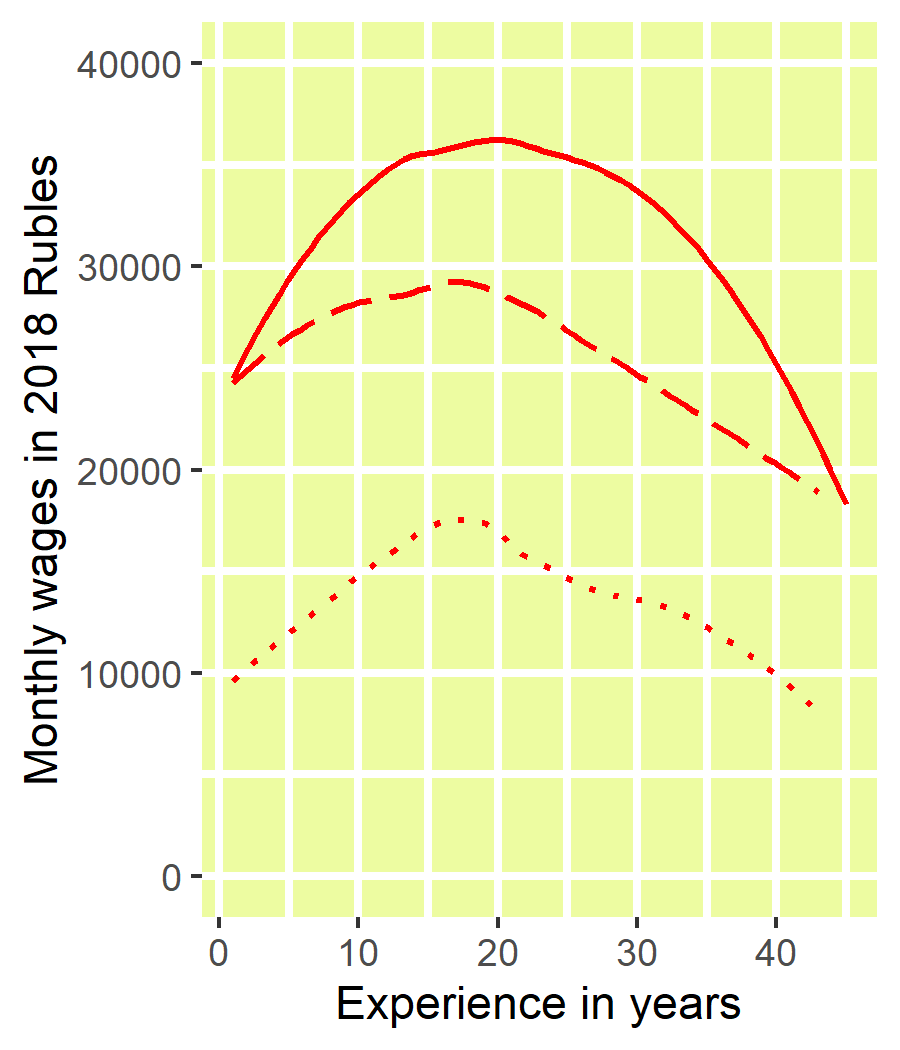
\includegraphics[width=150pt]{dp01_he.png}
			% plot 1
			\subcaption{Higher Education}\label{fig:1.1a}
		\end{minipage}
		\hfill
		\begin{minipage}[b]{.3\linewidth}
			\centering
			\hspace*{-0.7in}
			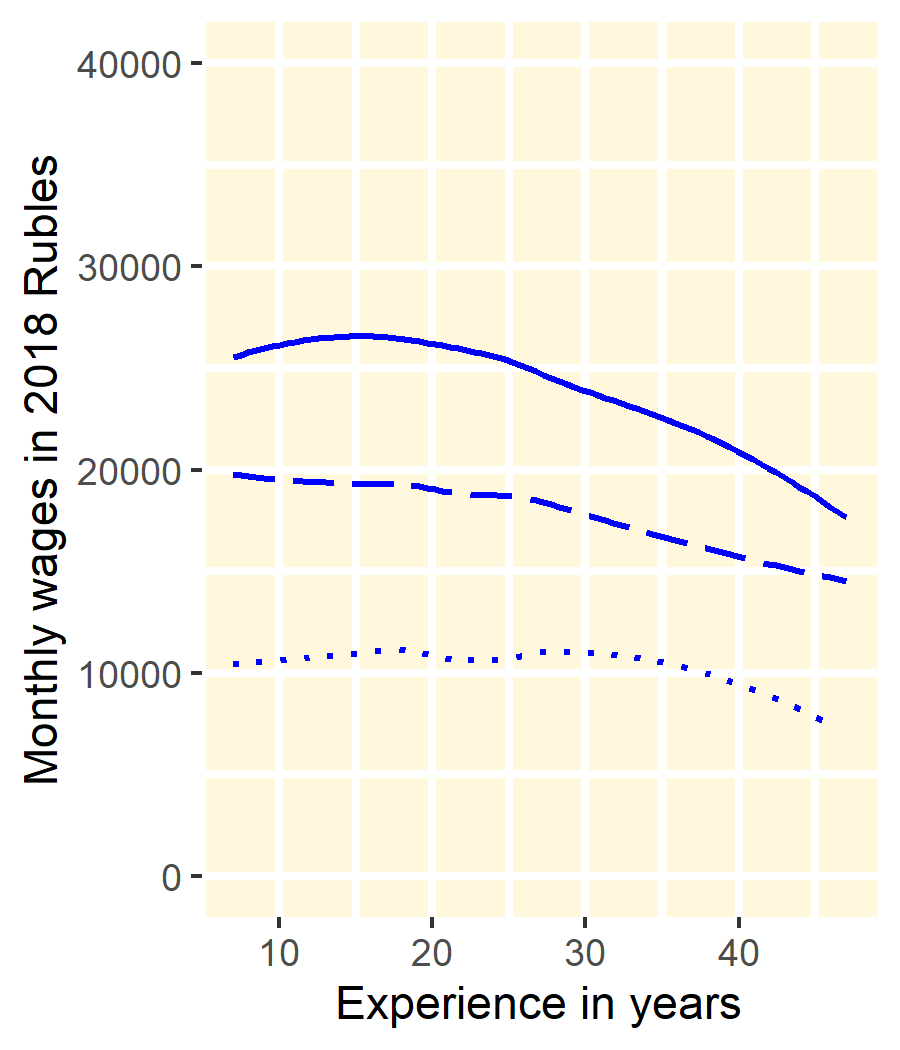
\includegraphics[width=150pt]{dp01_ve.png}
			% plot 2
			\subcaption{Vocational Education}\label{fig:1.1b}
		\end{minipage}
		\hfill
		\begin{minipage}[b]{.3\linewidth}
			\centering
			\hspace*{-0.7in}
			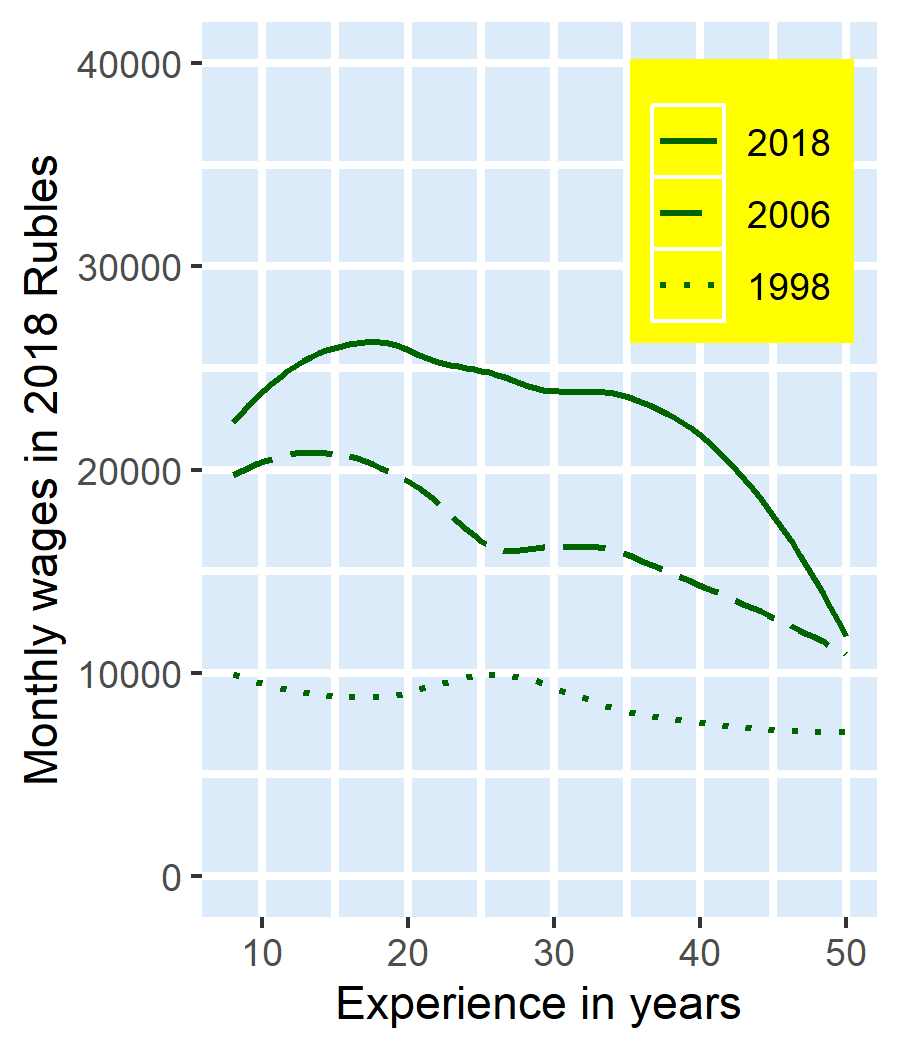
\includegraphics[width=150pt]{dp01_se.png}
			% plot 2
			\subcaption{Secondary Education}\label{fig:1.1c}
		\end{minipage}
		\caption{Neuman-Weiss vintage effects by education level from RLMS Rounds 1998, 2006 and 2018}\label{fig:1.1}
	\end{figure}
	
Putting the curves together by year (Figure \ref{fig:1.2}) suggests that 
the premium for university education over the other two levels does narrow 
at higher levels of experience. In the figure, to accommodate the 
relatively lower wage levels of 1998, the leftmost panel (Figure 
\ref{fig:1.2a}) is slightly compressed compared to the other two panels. 
The  converging tendency between levels of education would suggest that 
depreciation is indeed higher for university graduates. In the next two 
subsections, we present a more rigorous quantitative treatment of this 
issue, using a variant of Neuman-Weiss developed by \citet{Murillo_2006} 
and an alternative approach developed by \citet{Arrazola_2005}.

\begin{figure}[htbp!]
\hspace{0.35in}
		\begin{minipage}[b]{.3\linewidth}
			\centering
			\hspace*{-0.7in}
			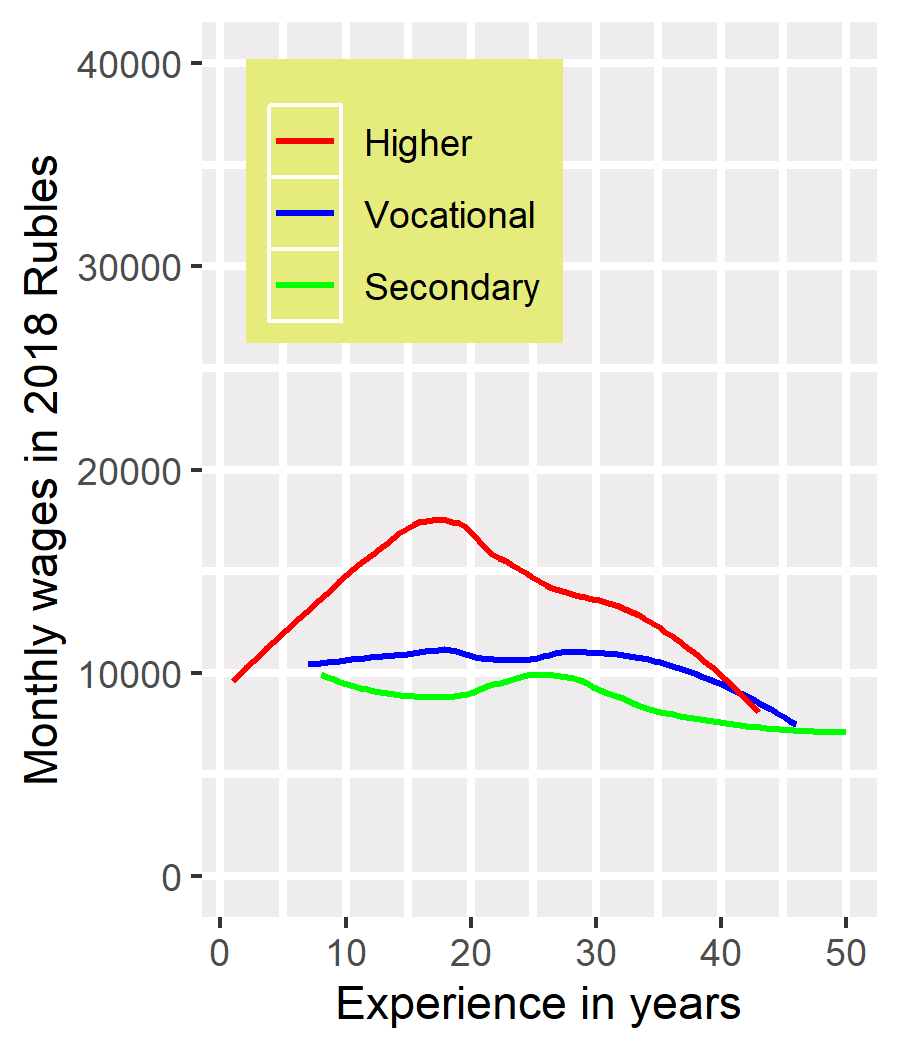
\includegraphics[width=150pt]{dp01_98.png}
			% plot 1
			\subcaption{1998}\label{fig:1.2a}
		\end{minipage}
		\hfill
		\begin{minipage}[b]{.3\linewidth}
			\centering
			\hspace*{-0.7in}
			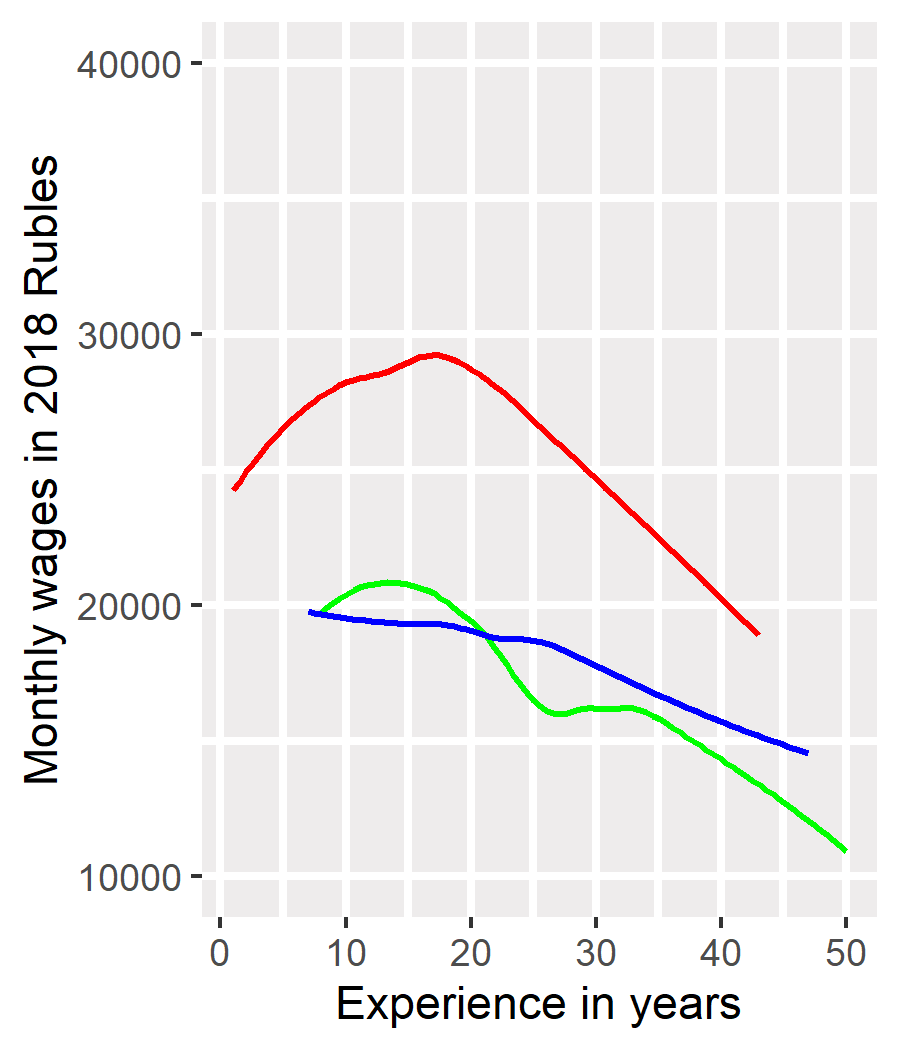
\includegraphics[width=150pt]{dp01_06.png}
			% plot 2
			\subcaption{2006}\label{fig:1.2b}
		\end{minipage}
		\hfill
		\begin{minipage}[b]{.3\linewidth}
			\centering
			\hspace*{-0.7in}
			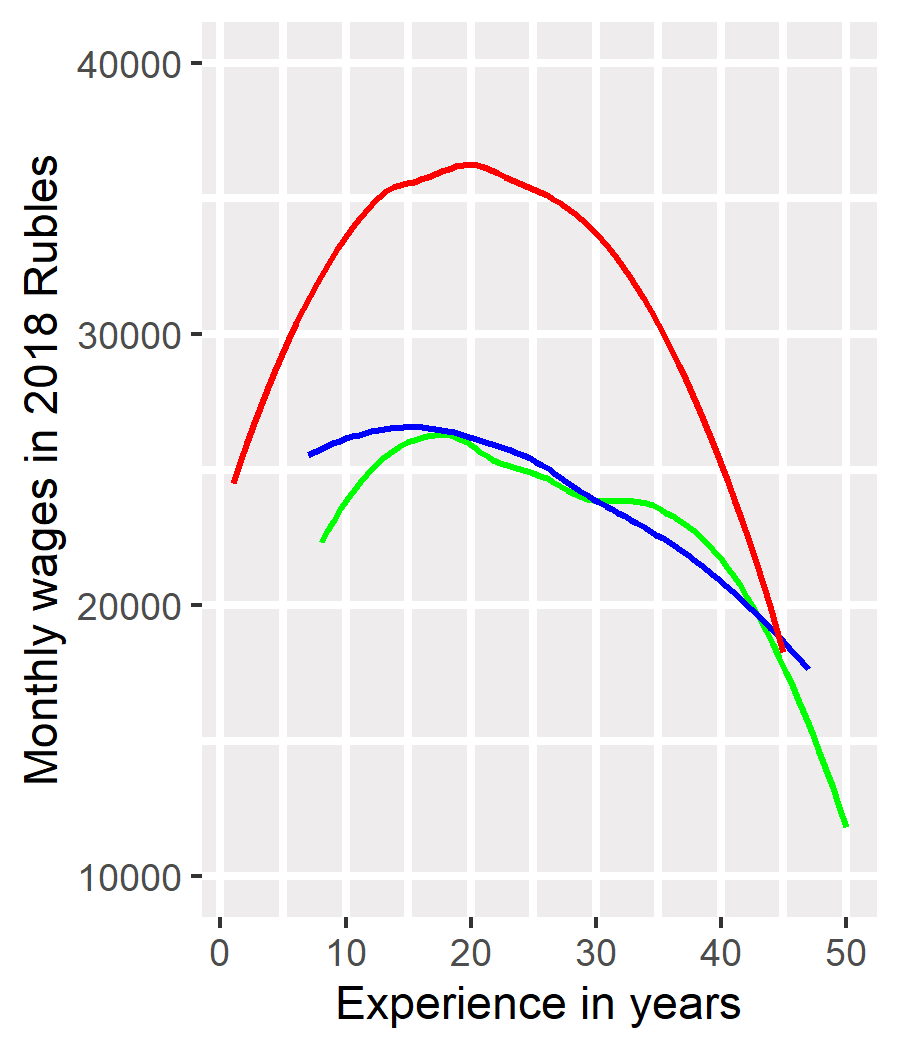
\includegraphics[width=150pt]{dp01_18.png}
			% plot 2
			\subcaption{2018}\label{fig:1.2c}
		\end{minipage}
		\caption{Neuman-Weiss vintage effects by Year from RLMS Rounds 1998, 2006 and 2018}\label{fig:1.2}
	\end{figure}



\subsection{Differential Depreciation Affecting Education and Training}
	
\citet{Murillo_2006} implemented a variation of the Neuman and Weiss model with a focus on empirical implementation to Spain. We follow the Murillo notation in the implementation of the model, which begins with the following earnings equation: 
\begin{flalign}\label{eq:2.1} 
log(W_{T}) = \alpha + \beta_{1}KS_{T} +  \beta_{2}KE_{T} &&
\end{flalign}
\noindent
where $W$ represents earnings, $KS$ the stock of human capital derived from schooling of $S$ years, and $KE$ the stock of human capital acquired from on the job training or experience, and $T$ indexes the number of experience years since completing formal education. In this set-up, the parameters $\beta_1$ and $\beta_2$ are the productivity parameters for the respective parts of the stock of human capital. Both are assumed to suffer from depreciation or the loss of productive value. At this stage, we do not distinguish between the causes (internal or external) of this loss. The path of the stock of human capital due to education is given by 
\begin{flalign}\label{eq:2.2} 
KS_{T} = S + hTS &&
\end{flalign} 
\noindent
where $h$ is the rate of loss of the stock. The next equation for the loss of stock gained from experience is a bit more complicated. The stock from schooling, $S$ is taken to be fixed at the end of the full-time schooling period and the beginning of the working period. However, experience is being built up every year at the same time as the capital acquired from previous experience depreciates. 
\begin{flalign}\label{eq:2.3} 
KE_{T} = \{1 + (T-1)\cdot\gamma \} + \{1 + (T-2)\cdot\gamma \}  + \{1 + (T-3)\cdot\gamma \} + \ldots + \{1\}  && 
\end{flalign} 
\noindent
where $\gamma$ is the rate of loss applied every year. The equation can be simplified and summarized as
\begin{flalign}\label{eq:2.4} 
KE_{T} =  T + \gamma\cdot\{(T-1) + (T-2) + (T-3) + \ldots + 1\} = T + \gamma\cdot\frac{T^2}{2}   && 
\end{flalign} 
Substituting equations \ref{eq:2.2} and \ref{eq:2.4} into equation \ref{eq:2.1}, we get
\begin{flalign}\label{eq:2.5} 
log(W) = \alpha +  \beta_{1}S +  \beta_{1}hTS + \beta_{2}T + \frac{\beta_{2}\gamma}{2}T^{2} =  \alpha +  \beta_{1}S + \pi_{1}TS + \beta_{2}T + \pi_{2}T^{2} && 
\end{flalign} 
\noindent
where $\pi_{1} = \beta_{1}h$ and $\pi_{2} = \frac{\beta_{2}\gamma}{2}$. 
\vspace{2pt}
\noindent
From \ref{eq:2.5}, the depreciation rate during $T$ years applied to schooling can be computed as $\pi_{1}S $ and the depreciation rate applied to experience as $ 2\pi_{2}T$.
\vspace{-5pt}
\subsubsection{Estimation Results}

We analyze separately six years that represent the ends (1994 and 2018), the 
diffused peak (2003 and 2006), and halfway points to the ends (1998 and 
2012) of the inverted-U shape shown in Appendix Figure \ref{fig:7.6}. Table \ref{tab:1.1} shows OLS estimation results of equation \ref{eq:2.5} run on the whole sample of the RLMS observations. The idea is to examine the role played by changes in depreciation to explain the observed pattern of variation in the rates of return over the time period}. 

Using the coefficient estimates derived from Table \ref{tab:1.1}, we compute the depreciation rate during $T$ years applied to schooling as $\pi_{1}S $ and the depreciation rate applied to experience as $ 2\pi_{2}T$, evaluating the expression at the mean level of schooling. Table \ref{tab:1.2} reports the depreciation rate values so calculated with the corresponding sample means. The table shows an interesting U-shaped pattern in the depreciation rate for human capital, attributable mainly to the depreciation rate associated with experience. The depreciation rate associated with education has been declining steadily and did not pick up again as measured with the given data. The depreciation rate associated with experience declined at first and then picked up again. 

Further work is required, including computation of the depreciation rates 
at levels other than the mean values. At this stage, the findings raise 
some interesting questions which needs to be addressed by further research. 
In the period from 1994 to 2006, the depreciation rate appears to be 
declining, just as the rates of return were on an ascending curve. As both 
kinds of depreciation (for experience and education) were declining, it is 
possible that the main cause was in the labor market experience rather than 
in the education system. Since the peak of earnings premiums in the 
2003-2006 period, as returns to education have declined, we see that the 
depreciation rates associated with experience have started climbing back, 
but depreciation rates associated with education have declined to null and 
not reverted. It is tempting to claim that this indicates a qualitative 
improvement in the skills provided by the education system, but further 
investigation is warranted before making such a claim. We explore next an 
alternative computation of the depreciation rate. 

%\begin{tabular}{p{1in}p{2in}}

%\vspace{1in}

% \end{tabular}


\setlength{\tabcolsep}{2pt}
\begin{table}[htbp!]
	\centering 
	\caption{Results of Estimating Human Capital Depreciation for the Whole Sample, RLMS} 
	\label{tab:1.1}
	\begin{tabular}{@{\extracolsep{3pt}}lcccccc} 
		\\[-1.8ex]\hline 
		\hline \\[-1.8ex] 
		& \textbf{1994} & \textbf{1998} & \textbf{2003} & \textbf{2006} & \textbf{2012} & \textbf{2018} \\ 
		\\[-1.8ex] & (1) & (2) & (3) & (4) & (5) & (6)\\ 
		\hline \\[-1.8ex] 
		Constant & 10.266$^{***}$ & 4.720$^{***}$ & 6.762$^{***}$ & 7.854$^{***}$ & 8.889$^{***}$ & 9.205$^{***}$ \\ 
		& (0.301) & (0.258) & (0.221) & (0.181) & (0.128) & (0.158) \\ 
		& & & & & & \\ 
		Educ, years ($S$) & 0.113$^{***}$ & 0.116$^{***}$ & 0.094$^{***}$ & 0.074$^{***}$ & 0.054$^{***}$ & 0.053$^{***}$ \\ 
		& (0.020) & (0.017) & (0.015) & (0.012) & (0.008) & (0.010) \\ 
		& & & & & & \\ 
		Educ X Exper ($TS$) & $-$0.001$^{*}$ & $-$0.001$^{*}$ & $-$0.00005 & 0.0003 & 0.0003 & 0.0001 \\ 
		& (0.001) & (0.001) & (0.001) & (0.0005) & (0.0003) & (0.0004) \\ 
		& & & & & & \\ 
		Exper($T$) & 0.053$^{***}$ & 0.044$^{***}$ & 0.016 & $-$0.001 & 0.012$^{*}$ & 0.023$^{***}$ \\ 
		& (0.015) & (0.013) & (0.011) & (0.009) & (0.007) & (0.008) \\ 
		& & & & & & \\ 
		Exper squared ($T^2$) & $-$0.001$^{***}$ & $-$0.001$^{***}$ & $-$0.0004$^{***}$ & $-$0.0002$^{*}$ & $-$0.001$^{***}$ & $-$0.001$^{***}$ \\ 
		& (0.0002) & (0.0001) & (0.0001) & (0.0001) & (0.0001) & (0.0001) \\ 
		& & & & & & \\ 
		\hline \\[-1.8ex] 
		Observations & 3,037 & 3,100 & 3,856 & 4,800 & 7,417 & 6,112 \\ 
		R$^{2}$ & 0.043 & 0.058 & 0.068 & 0.078 & 0.088 & 0.071 \\ 
		Adjusted R$^{2}$ & 0.042 & 0.057 & 0.067 & 0.077 & 0.087 & 0.071 \\ 
		Residual Std. Error & 0.934 & 0.800 & 0.782 & 0.715 & 0.666 & 0.617 \\ 
		F Statistic & 34.062$^{***}$ & 47.678$^{***}$ & 69.846$^{***}$ & 101.053$^{***}$ & 177.952$^{***}$ & 117.104$^{***}$ \\ 
		\hline 
		\hline \\[-1.8ex] 
		\textit{Note:}  & \multicolumn{6}{r}{$^{*}$p$<$0.1; $^{**}$p$<$0.05; $^{***}$p$<$0.01} \\ 
	\end{tabular} 
\end{table}

\newpage

%\begin{tabular}{p{1in}p{2in}}
%\textcolor{white}{Silliest hack ever}
%\end{tabular}


\begin{center}
\captionof{table}{Average Depreciation Rate by Years}\label{tab:1.2}
\keepXColumns
\begin{tabularx}{\textwidth}{@{\extracolsep{5pt}}rlrrrrrrc}
		\hline
\multicolumn{9}{l}{\textbf{Panel A: Whole Sample}} \\
\hline
			& \textbf{Statistic} & \textbf{1994} & \textbf{1998} & \textbf{2003} & \textbf{2006} & \textbf{2012} & \textbf{2018} &  \\ 
		\hline
		1 & Experience, mean   & 21.41 & 22.32 & 22.20 & 22.24 & 22.52 & 22.52 & \\
		2 & Education, mean & 12.70 & 12.69 & 12.79 & 12.79 & 12.95 & 13.27 &\\
		\midrule
		3 & DR Experience, \% & 1.87 & 1.55 & 1.04 & 0.50 & 1.37 & 1.63 & 
\graph{1}{1}{all2-1} \\ 
		4 & DR Education, \% & 2.80 & 2.71 & 0.11 & 0.00 & 0.00 & 0.00 &
\graph{1}{1}{all2-2} \\ 
		5 & DR Human Capital, \% & 4.67 & 4.26 & 1.15 & 0.50 & 1.37 & 1.63 & 
\graph{1}{1}{all2-3}\\ 
		\hline
\end{tabularx}
%\par\noindent
\begin{tabularx}{\textwidth}{@{\extracolsep{5pt}}rlrrrrrrc}
		\hline
\multicolumn{9}{l}{\textbf{Panel B: Female Sample}} \\
		\hline
  1 & Experience, mean & 21.36 & 22.09 & 22.34 & 22.33 & 22.69 & 22.67 & \\  
  2 & Education, mean & 12.76 & 12.85 & 12.98 & 13.05 & 13.24 & 13.58 & \\ 
  3 & DR Experience, \% & 2.46 & 2.57 & 1.62 & 0.78 & 1.23 & 1.52 & 
\graph{1}{1}{female2-1} \\  
  4 & DR Education, \% & 3.81 & 5.31 & 3.97 & 0.00 & 0.00 & 0.00 & 
\graph{1}{1}{female2-2} \\
  5 & DR Human Capital, \% & 6.27 & 7.88 & 5.59 & 0.78 & 1.23 & 1.52 & 
\graph{1}{1}{female2-3} \\ 
   \hline
\end{tabularx}
\begin{tabularx}{\textwidth}{@{\extracolsep{5pt}}rlrrrrrrc}
		\hline
\multicolumn{9}{l}{\textbf{Panel C: Male Sample}} \\
  \hline
1 & Experience, mean & 21.47 & 22.58 & 22.02 & 22.14 & 22.31 & 22.34 & \\ 
  2 & Education, mean & 12.62 & 12.50 & 12.57 & 12.47 & 12.61 & 12.91 & \\  
  3 & DR Experience, \% & 1.83 & 1.08 & 0.80 & 0.67 & 2.23 & 1.91 & 
\graph{1}{1}{male2-1} 
\\ 
  4 & DR Education, \% & 3.96 & 2.74 & 0.91 & 0.00 & 0.00 & 0.00 & 
\graph{1}{1}{male2-2} 
\\ 
  5 & DR Human Capital, \% & 5.78 & 3.82 & 1.71 & 0.67 & 2.23 & 1.91 &
\graph{1}{1}{male2-3} 
\\ 
   \hline
\end{tabularx}
\end{center}

\setcounter{table}{2} % to avoid tabularx counting subtables as tables


\subsection{Depreciation of Human Capital using Non-Linear Least Squares}

\citet{Arrazola_2005} developed an alternative approach the issue of human capital depreciation with a first principles approach regarding the formation of human capital, providing an empirical estimation for Spain.  A number of other authors have replicated Arrazola's approach. In this paper, we follow the notation adopted by Sylvain Weber, who estimated depreciation rates for Switzerland (\citet{Weber_2008} and \citet{Weber_2011}). Weber starts with the definition of $s_{t}$ -- the time fraction invested into the generation of new human capital by a person at age $t$. Relying on a human capital theory implication about the decline of $s_{t}$ over the life cycle, Weber shows that the complete path of $s_{t}$ is written as follows:

\begin{flalign}\label{eq:2.6} 
s_{t}=\left\{\begin{array}{ll}
{0} & {\text { if } t<6} \\
{1} & {\text { if } 6 \leq t<S^{\star}} \\
{\alpha-\frac{\mathlarger{\alpha}}{T-S^{*}} \cdot\left(t-S^{\star}\right)=\alpha \cdot\left(1-\frac{X_{t}}{L}\right)} & {\text { if } S^{\star} \leq t \leq T}
\end{array}\right.
\end{flalign}


\noindent
where $\alpha$ is a parameter, $S^{*}$ is the age when schooling life ends and the working one begins, $T$ is the retirement age, $L = T - S^{*}$ is the total working life length, $X_{t} = t - S^{*}$ is experience. Schooling duration is equal to $S^{*} - 6$.

The model then utilizes the standard human capital theory specification that potential earnings $E_{t}$ are exponentially related to the human capital stock:

\begin{flalign}\label{eq:2.7} 
E_{t}=W \cdot \exp \left(\beta_{K} K_{t}+\beta_{Z} Z_{t}\right)
\end{flalign}



\noindent
where $W$ is a return per period on a unit of earnings capacity, $K_{t}$  is the stock of human capital at time $t$, $Z_{t}$ is a set of observable attributes supposed to influence on earnings, and $K, Z$ are the parameters of interest. The stock of human capital in period $t$ can be estimated as the sum of the stock from the previous period minus the loss due to depreciation plus the quantity generated during the $t_{th}$ period:

\begin{flalign}\label{eq:2.8} 
K_{t}=K_{t-1}-\delta \cdot K_{t-1}+\Delta K_{t}=(1-\delta) \cdot K_{t-1}+\Delta K_{t}
\end{flalign}

By recursion, an expression for $K_{t}$ as a function of the human capital stock acquired at the end of formal education $K_{S}$ is given by:

\begin{flalign}\label{eq:2.9}
K_{t}=(1-\delta)^{t} \cdot K_{S}+\sum_{j=S^{*}}^{t-1}(1-\delta)^{j} \cdot \Delta K_{t-j}
\end{flalign}

Taking the logarithms of the expression \ref{eq:2.7} and substituting $K_{t}$ by the equation \ref{eq:2.9} leads to:

\begin{flalign}\label{eq:2.10} 
\ln E_{t}=\ln W+\beta_{K} \cdot\left\{(1-\delta)^{t} \cdot K_{S}+\sum_{j=S^{*}}^{t-1}(1-\delta)^{j} \cdot \Delta K_{t-j}\right\}+\beta_{Z} Z_{t}
\end{flalign}

Next is the standard human capital relationship between observed and potential earnings. As only a proportion of $s_{t}$  of the human capital stock is  used in the actual production of earnings, observed earnings can be expressed by:

\begin{flalign}\label{eq:2.11} 
\begin{aligned}
&Y_{t}=\left(1-s_{t}\right) \cdot E_{t}\\
&\ln Y_{t}=\ln \left(1-s_{t}\right)+\ln E_{t}
\end{aligned}
\end{flalign}

Combining \ref{eq:2.10} and \ref{eq:2.11} results in:

\begin{flalign}\label{eq:2.12} 
\ln Y_{t}=\ln W+\beta_{K} \cdot\left\{(1-\delta)^{t} \cdot K_{S}+\sum_{j=S^{*}}^{t-1}(1-\delta)^{j} \cdot \Delta K_{t-j}\right\} + \beta_{Z} Z_{t} + \ln \left(1-s_{t}\right)
\end{flalign}

Finally, as the human capital stock at the end of education is related to the human capital received, there is a direct association between this stock and the schooling duration:

\begin{flalign}\label{eq:2.13} 
K_{S}=S
\end{flalign}

The production of new human capital $K_{t}$ depends on the portion of time devoted to this activity:

\begin{flalign}\label{eq:2.14} 
\Delta K_{t}=s_{t}=\left\{\begin{array}{ll}
{0} & {\text { if } t<6} \\
{1} & {\text { if } 6 \leq t<S^{\star}} \\
{\alpha \cdot\left(1-\frac{X_{t}}{L}\right)} & {\text { if } S^{*} \leq t \leq T}
\end{array}\right.
\end{flalign}

Using \ref{eq:2.8} and \ref{eq:2.11} to express $K_{S}$ as a sum of the human capital quantities produced during schooling, the result is:

\begin{flalign}\label{eq:2.15} 
K_{S} \stackrel{(3)}{=} \sum_{j=0}^{S^{*}}(1-\delta)^{j} \cdot \Delta K_{S^{*}-j} \stackrel{(9)}{=} \sum_{j=6}^{S^{*}}(1-\delta)^{j}
\end{flalign}

Substituting \ref{eq:2.13} and \ref{eq:2.14} into \ref{eq:2.12}, adding an error term and an individual subscript $i$  provides the equation that can be estimated using non-linear least squares (NLS):

\begin{multline}\label{eq:2.16} 
\ln Y_{i t}= \ln W+\beta_{K} \cdot\left\{(1-\delta)^{X_{i t}} \cdot S_{i}+\alpha \cdot \frac{1-(1-\delta)^{X_{i t}}}{\delta}\right.\cdot\\
\left.\left(1+\frac{1-\delta}{\delta \cdot L_{i}}\right)-\frac{\alpha \cdot X_{i t}}{\delta \cdot L_{i}}\right\}+\ln \left\{1-\left(\alpha-\frac{\alpha}{L_{i}} \cdot X_{i t}\right)\right\}+\beta_{Z} \cdot Z_{i t}+u_{i t}
\end{multline}

\noindent
where $t$ shows a time period, $\ln Y$ is a logarithm of the observed 
earnings, $\ln W$ is a logarithm of a return per certain period on a unit 
of earnings capacity, $\beta_{K}$ is the effect of the human capital stock 
on earnings, $\beta_{Z}$ is the effect of other covariates in the model on 
earning, $\delta$ is the human capital depreciation rate, $X_{i t}$ is the 
labor market experience, $L_{i}$ is the total working life length, $\alpha$ 
is a parameter reflecting the share of time invested in training 
immediately after leaving school, $Z_{i t}$ is a set of observable 
attributes hypothesized to have an impact on earnings, $u_{i t}$ is an 
error term. In this model, the share of time invested in training after 
school starts at alpha and declines to zero at the end of the working 
period. 

The parameter alpha is notional, a parameter that helps to explain 
observed empirical patterns - it should not be considered literally as time 
devoted in explicit training programs. Post-schooling increments to human 
capital can also be understood by examining another group of workers that 
is not included in the model of Equation \ref{eq:2.16}.  \cite{Mincer_1982} 
document a most interesting phenomenon with regard to workers who leave and 
then return to the workforce: ``It is rather surprising to find that 
returnees from the non-market appear to incur greater job investments upon 
return to the market than do stayers of the same age and education.'' The 
authors also refer to a similar phenomenon of re-investment amongst 
international migrants - they attribute the significant increases in wage 
earnings in the first years of international migrants to the USA to post 
school reinvestment. The authors characterize such investment as a 
re-adaptation or repair of skills. It is straightforward to extend this 
process of continuous `repair of skill damage' as being a phenomenon that 
affects all workers, not just intermittent workers or migrants. 


Table \ref{tab:1.3} reports empirical findings for the estimation of the 
\ref{eq:2.16} equation using NLS with robust standard errors for the same 
range of years as presented in the previous section. Unlike that earlier 
model, the Arrazola model does not allow for a different treatment of 
depreciation of human capital acquired from schooling or from experience - 
only a single $\delta$ (depreciation rate of the human capital) parameter 
is estimated. However, the model does allow the identification of an  
$\alpha$ parameter (related to post-school investment in human capital). 

\newpage


\begin{center}
	\captionof{table}{Non-Linear Lest Squares estimated for range of years}
	\label{tab:1.3}
	\keepXColumns
	\begin{tabularx}{\textwidth}{clccccccc}
		\hline
		\multicolumn{9}{l}{\textbf{Panel A: Whole Sample}} \\
		\hline
		& Parameter & 1994 & 1998 & 2003 & 2006 & 2012 & 2018 & \\ 
		\hline
		 & lnW & 10.4780 & 4.8622 & 6.7305 & 7.8405 & 8.4104 & 8.8524 & \\ 
		 &  & (0.1913) & (0.1646) & (0.1409) & (0.0838) & (0.0787) & (0.0885) & \\ 
		 & bk & 0.1453 & 0.1429 & 0.1144 & 0.0723 & 0.1382 & 0.1487 & \\ 
		 &  & (0.0167) & (0.0144) & (0.0140) & (0.0106) & (0.0087) & (0.0086) & \\ 
		 & delta & 0.0246 & 0.0208 & 0.0093 & -0.0040 & 0.0369 & 0.0459 & 
		\graph{1}{1}{C:/Country/Russia/Data/SEASHELL/SEABYTE/Edreru/wp1/sparklines/Weber_sprk_all2-1}\\ 
		 &  & (0.0052) & (0.0043) & (0.0050) & (0.0058) & (0.0043) & (0.0051) & \\ 
		 & alpha & 0.4798 & 0.3860 & 0.1352 & -0.1690 & 0.4972 & 0.6686 & 
		\graph{1}{1}{C:/Country/Russia/Data/SEASHELL/SEABYTE/Edreru/wp1/sparklines/Weber_sprk_all2-2}\\ 
		 &  & (0.0912) & (0.0790) & (0.0911) & (0.0950) & (0.0601) & (0.0533) & \\ 
		 & Sample size & 3037 & 3100 & 3856 & 4800 & 7417 & 6112 & \\ 
		\hline
\end{tabularx}

\begin{tabularx}{\textwidth}{clccccccc}
		\hline
		\multicolumn{9}{l}{\textbf{Panel B: Female Sample}} \\
		\hline
		& Parameter & 1994 & 1998 & 2003 & 2006 & 2012 & 2018 & \\ 
		\hline
		 & lnW & 10.1580 & 4.1353 & 5.7238 & 6.9251 & 7.9143 & 8.4131 & \\ 
		 &  & (0.2447) & (0.2124) & (0.1973) & (0.1663) & (0.1136) & (0.1275) & \\ 
		 & bk & 0.1524 & 0.1818 & 0.1702 & 0.1321 & 0.1329 & 0.1330 & \\ 
		 &  & (0.0196) & (0.0163) & (0.0158) & (0.0149) & (0.0104) & (0.0103) & \\ 
		 & delta & 0.0275 & 0.0260 & 0.0156 & 0.0065 & 0.0197 & 0.0249 & 
		\graph{1}{1}{C:/Country/Russia/Data/SEASHELL/SEABYTE/Edreru/wp1/sparklines/Weber_sprk_f2-1}\\ 
		 &  & (0.0060) & (0.0042) & (0.0038) & (0.0044) & (0.0036) & (0.0036) & \\ 
		 & alpha & 0.5889 & 0.5408 & 0.3466 & 0.0900 & 0.3354 & 0.4628 & 
		\graph{1}{1}{C:/Country/Russia/Data/SEASHELL/SEABYTE/Edreru/wp1/sparklines/Weber_sprk_f2-2}\\ 
		 &  & (0.0974) & (0.0749) & (0.0763) & (0.0862) & (0.0659) & (0.0609) & \\ 
		 & Sample size & 1645 & 1667 & 2093 & 2630 & 4057 & 3312 & \\ 
		\hline	
\end{tabularx}

\begin{tabularx}{\textwidth}{clccccccc}
		\hline
		\multicolumn{9}{l}{\textbf{Panel C: Male Sample}} \\
		\hline
		& Parameter & 1994 & 1998 & 2003 & 2006 & 2012 & 2018 & \\ 
		\hline
		 & lnW & 10.4992 & 5.1267 & 7.3195 & 8.1556 & 8.2117 & 8.8384 & \\ 
		 &  & (0.2880) & (0.2420) & (0.1530) & (0.1158) & (0.1195) & (0.1213) & \\ 
		 & bk & 0.1697 & 0.1425 & 0.0845 & 0.0725 & 0.2206 & 0.1784 & \\ 
		 &  & (0.0244) & (0.0215) & (0.0180) & (0.0163) & (0.0111) & (0.0118) & \\ 
		 & delta & 0.0261 & 0.0168 & -0.0020 & 0.0015 & 0.0595 & 0.0511 & 
		\graph{1}{1}{C:/Country/Russia/Data/SEASHELL/SEABYTE/Edreru/wp1/sparklines/Weber_sprk_m2-1}\\ 
		 &  & (0.0067) & (0.0059) & (0.0082) & (0.0095) & (0.0063) & (0.0069) & \\ 
		 & alpha & 0.4625 & 0.2669 & -0.1351 & -0.1196 & 0.8161 & 0.7312 & 
		\graph{1}{1}{C:/Country/Russia/Data/SEASHELL/SEABYTE/Edreru/wp1/sparklines/Weber_sprk_m2-2}\\ 
		 &  & (0.1278) & (0.1162) & (0.1362) & (0.1475) & (0.0484) & (0.0663) & \\ 
		 & Sample size & 1392 & 1433 & 1763 & 2170 & 3360 & 2800 & \\ 
		\hline	
\end{tabularx}
\end{center}

\setcounter{table}{3} % to avoid tabularx counting subtables as tables

The sparklines in Table \ref{tab:1.3} indicates a similar roughly U-shaped  
pattern for depreciation as reported in Table \ref{tab:2.2}, with 
depreciation of human capital first declining and then increasing again. 
This supports the narrative that the observed increase and then decrease in 
returns to education in the Russian Federation may be explained through the 
effect of depreciation. The  exact magnitudes of estimated depreciation in 
the two tables do not match - while the range of depreciation is similar - 
between 2\% to 5\%, the 2018 figures indicate a higher level in Table 
\ref{tab:2.3}. 

\vspace{3pt}

An intriguing finding concerns the difference in depreciation rates between female and male workers. The conventional human capital logic holds that women typically face longer periods outside of the labor market because of child-bearing and child-rearing responsibilities. Absence from the labor market would lead to higher levels of depreciation amongst women. In the case of the Russian Federation, the estimates of both Table \ref{tab:2.2} and Table \ref{tab:2.3} reflect this pattern in the first half of the period, up until the estimates for 2006. Around the time of the peak in returns, the depreciation rate drops to zero for both men and women, but in the subsequent period, the depreciation rate for men appears to be higher than the rate for women. The fact that both methodologies reflect this pattern indicates a real phenomenon, rather than a statistical artefact, and something to be explored further. 

\vspace{3pt}

Finally, a word about the $\alpha$ parameter, which is an indicator of post-schooling investment in human capital. This parameter also shows a similar tendency as the depreciation rate, meaning a decline to zero and a subsequent  increase. As with depreciation, the first half shows a higher $\alpha$ for female workers until it drops to zero for both males and females at the time of peak returns, and in the subsequent period the $\alpha$ parameter level is higher for males. 

\vspace{3pt}

Adopting a strategy utilized by (\citet{Weber_2008}) and modifying the approach to fit the Russian context, Table \ref{tab:1.4} provides four alternative specifications displayed separately by gender. The four models portray the following combinations regarding the $\alpha$  and $\delta$ parameters: \textit{Model I} - both $\alpha$ and $\delta$ are constant across education levels; \textit{Model II} - $\alpha$ is constant, $\delta$ varies; \textit{Model III} - $\alpha$ varies, $\delta$ is constant, \textit{Model IV} - both $\alpha$ and $\delta$ vary across education levels.

\vspace{3pt}

Model I - the base model, has already been presented in Table \ref{tab:1.3} 
and is shown again as part of Table \ref{tab:1.4} only for easy reference. 
Model II, allows the $\delta$ parameter to vary across education levels; 
Model III allows the $\alpha$ parameter to vary across education levels; 
and finally Model IV allows both parameters to vary by education level. The 
estimates indicate the absence of depreciation effects by educational 
level. Weber had found for Switzerland  that depreciation is higher for 
vocational education, and provided the explanation that vocational 
education skills tend to be more specific to jobs and careers. However, 
this finding is not replicated with the data for the Russian Federation. 
The statistically significant finding in Table \ref{tab:1.4} concerns the 
$\alpha$ parameter. Post-schooling investment in human capital for those 
with vocational education is not different from those with secondary 
education, but university education brings with it a higher level of the 
$\alpha$ parameter, for both male and female workers. 


\setlength{\tabcolsep}{2pt}
\begin{table}[htbp!]\centering
	\def\sym#1{\ifmmode^{#1}\else\(^{#1}\)\fi}
	\caption{Empirical Estimates for Females and Males, RLMS 2018}
	\label{tab:1.4}
	\begin{tabular}{l*{8}{c}}
		\toprule\\
		&\multicolumn{4}{c}{Females}&\multicolumn{4}{c}{Males}\\
		\cmidrule(lr){2-5}\cmidrule(lr){6-9}
		&\multicolumn{1}{c}{I}&\multicolumn{1}{c}{II}&\multicolumn{1}{c}{III}&\multicolumn{1}{c}{IV}&\multicolumn{1}{c}{I}&\multicolumn{1}{c}{II}&\multicolumn{1}{c}{III}&\multicolumn{1}{c}{IV}\\
		\cmidrule(lr){1-5}\cmidrule(lr){6-9}
		lnW&8.413\sym{***}&8.901\sym{***}&8.778\sym{***}&8.644\sym{***}&8.838\sym{***}&8.950\sym{***}&9.022\sym{***}&8.864\sym{***}\\
		&(0.127)&(0.319)&(0.0975)&(0.279)&(0.121)&(0.291)&(0.0925)&(0.221)\\
		\hline
		bk&0.133\sym{***}&0.111\sym{***}&0.125\sym{***}&0.129\sym{***}&0.178\sym{***}&0.177\sym{***}&0.183\sym{***}&0.179\sym{***}\\
		&(0.0103)&(0.0115)&(0.0105)&(0.0130)&(0.0118)&(0.0147)&(0.0122)&(0.0111)\\
		\hline
		delta&0.0249\sym{***}&&&&0.0511\sym{***}&&&\\
		&(0.00357)&&&&(0.00692)&&&\\
		\hline
		alpha&0.463\sym{***}&0.553\sym{***}&&&0.731\sym{***}&0.761\sym{***}&&\\
		&(0.0609)&(0.143)&&&(0.0663)&(0.124)&&\\
		\hline
		delta\_base&&0.0387\sym{*}&0.0355\sym{***}&0.0305\sym{*}&&0.0558\sym{**}&0.0597\sym{***}&0.0431\sym{**}\\
		&&(0.0181)&(0.00453)&(0.0134)&&(0.0185)&(0.00506)&(0.0144)\\
		\hline
		delta\_voc&&-0.00109&&-0.00128&&0.000258&&0.00694\\
		&&(0.00251)&&(0.00519)&&(0.00150)&&(0.00547)\\
		\hline
		delta\_uni&&-0.00699&&0.00198&&-0.00143&&0.00892\\
		&&(0.00610)&&(0.00805)&&(0.00333)&&(0.00728)\\
		\hline
		alpha\_base&&&0.448\sym{***}&0.424\sym{*}&&&0.698\sym{***}&0.498\sym{**}\\
		&&&(0.0728)&(0.172)&&&(0.0578)&(0.166)\\
		\hline
		alpha\_voc&&&0.0124&-0.0322&&&0.00828&0.144\\
		&&&(0.0442)&(0.128)&&&(0.0381)&(0.114)\\
		\hline
		alpha\_uni&&&0.208\sym{***}&0.206&&&0.157\sym{***}&0.307\sym{*}\\
		&&&(0.0533)&(0.134)&&&(0.0420)&(0.125)\\
		\hline
		\(N\)&3312&3312&3312&3312&2800&2800&2800&2800\\
		adj.\(R^{2}\)&0.082&0.085&0.091&0.091&0.096&0.096&0.106&0.107\\
		\textit{AIC}&6017.6&6006.2&5983.5&5987.1&4842.8&4844.9&4813.7&4814.6\\
		\textit{BIC}&6042.0&6042.8&6020.2&6035.9&4866.5&4880.5&4849.3&4862.1\\
		\bottomrule
		\multicolumn{9}{l}{\footnotesize Standard errors in parentheses}\\
		\multicolumn{9}{l}{\footnotesize \sym{*} \(p<0.05\), \sym{**} \(p<0.01\), \sym{***} \(p<0.001\)}\\
	\end{tabular}
\end{table}


\section{Further Exploration of Depreciation}
\subsection{Depreciation and the Gender dimension}

The previous section indicated an intriguing finding regarding depreciation 
and gender, with recent rounds of RLMS data indicating a higher level of 
depreciation for male workers, a possibly anomalous finding. This 
sub-section draws upon the literature regarding occupational gender 
segregation, the tendency for some jobs to be dominated by one gender, a 
phenomenon that has been studied in detail in labor markets around the 
world (\citet{Preston_1999} and \citet{Blau_2013}). Empirical application 
in the Russian Federation has examined trends regarding gender segregation 
in occupations 
(\citet{Klimova_2009},\citet{Klimova_2012},\citet{Kosyakova_2015}). The 
bulk of this literature is concerned with the issue of the possible 
inequities and inefficiencies arising from gender segregation. However, for 
the purpose of this paper is to exploit the presence in the data of 
occupational gender segregation to obtain insights into human capital 
depreciation.


In this section,we extend the Neuman and Weiss model of the previous 
section to compare the estimated depreciation rates between female- and 
male-dominated groups in various industries and occupations. The RLMS 2018 
database contains information about sector or industry and standardized 
ISCO-08 classification of jobs. These were used  to tag gender-based 
industrial sectors and occupations. The average female 
representation by sector was 54\%.  Using a range of $\pm$ 10\% from the 
average, a sector was marked as female-dominated if it contained more than 
64\% of women workers, and male-dominated if it contained less than 44\% of 
women workers. Neutral sectors occupied the middle of the distribution. 
Figure \ref{fig:2.1} visualizes this procedure; Table \ref{tab:2.1} maps 
title of sectors with female percentages in them. To generate 
gender-related occupations a similar tactic was applied based on the 
2-digit ISCO-08 classification (see Figure \ref{fig:2.2} and Table 
\ref{tab:2.2}). 

\begin{figure}[htbp!]
	\centering
	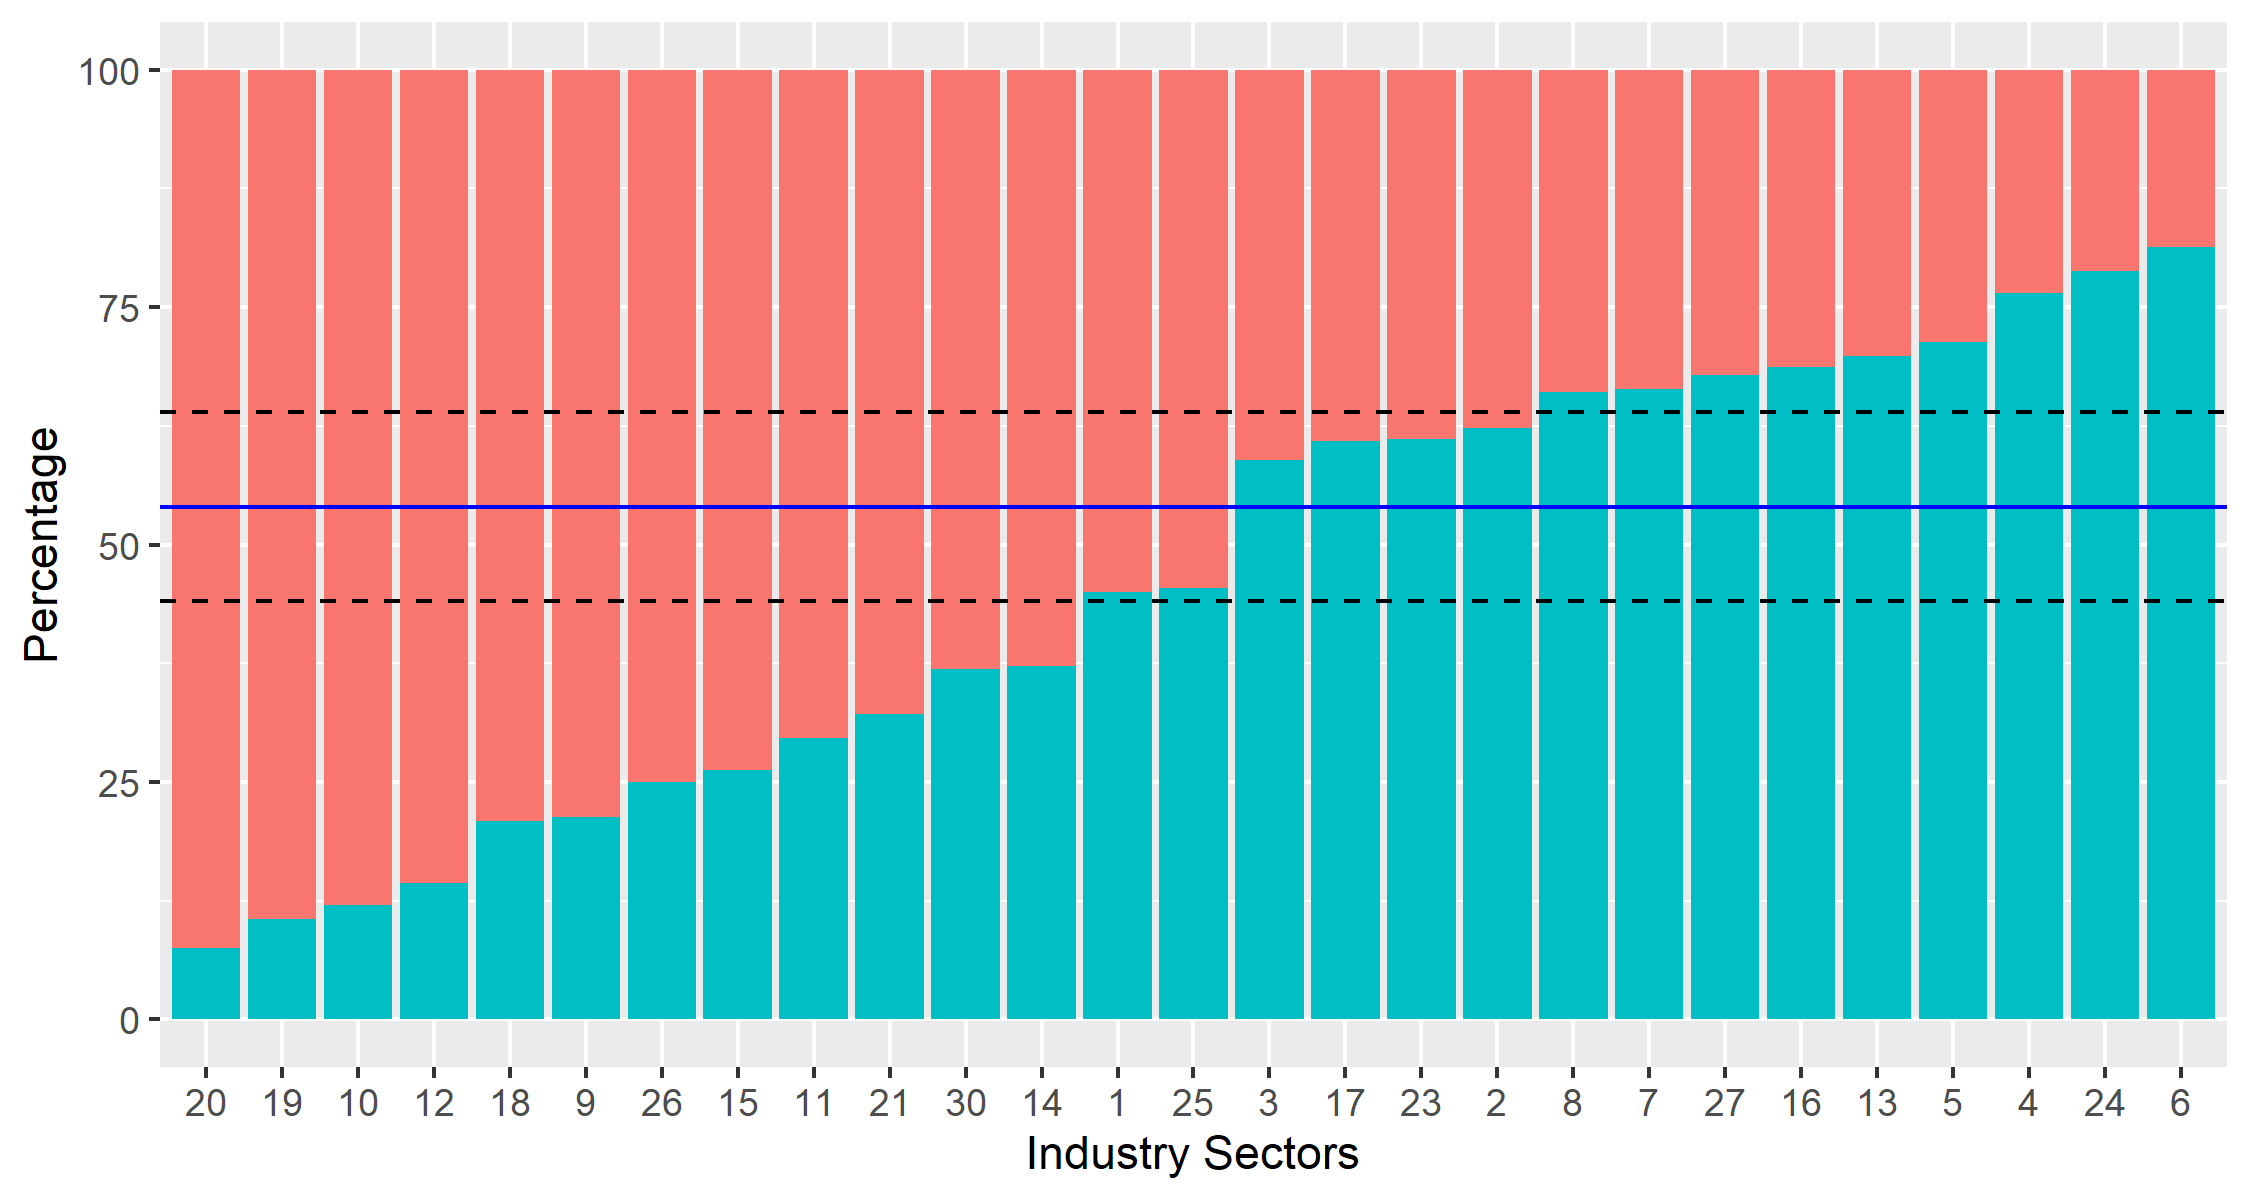
\includegraphics[width=400pt]{gen_ind18.png}
	\caption{Distribution of Employment in RLMS 2018 by Industry and Gender}\label{fig:2.1}
\end{figure}

\begin{figure}[htbp!]
	\centering
	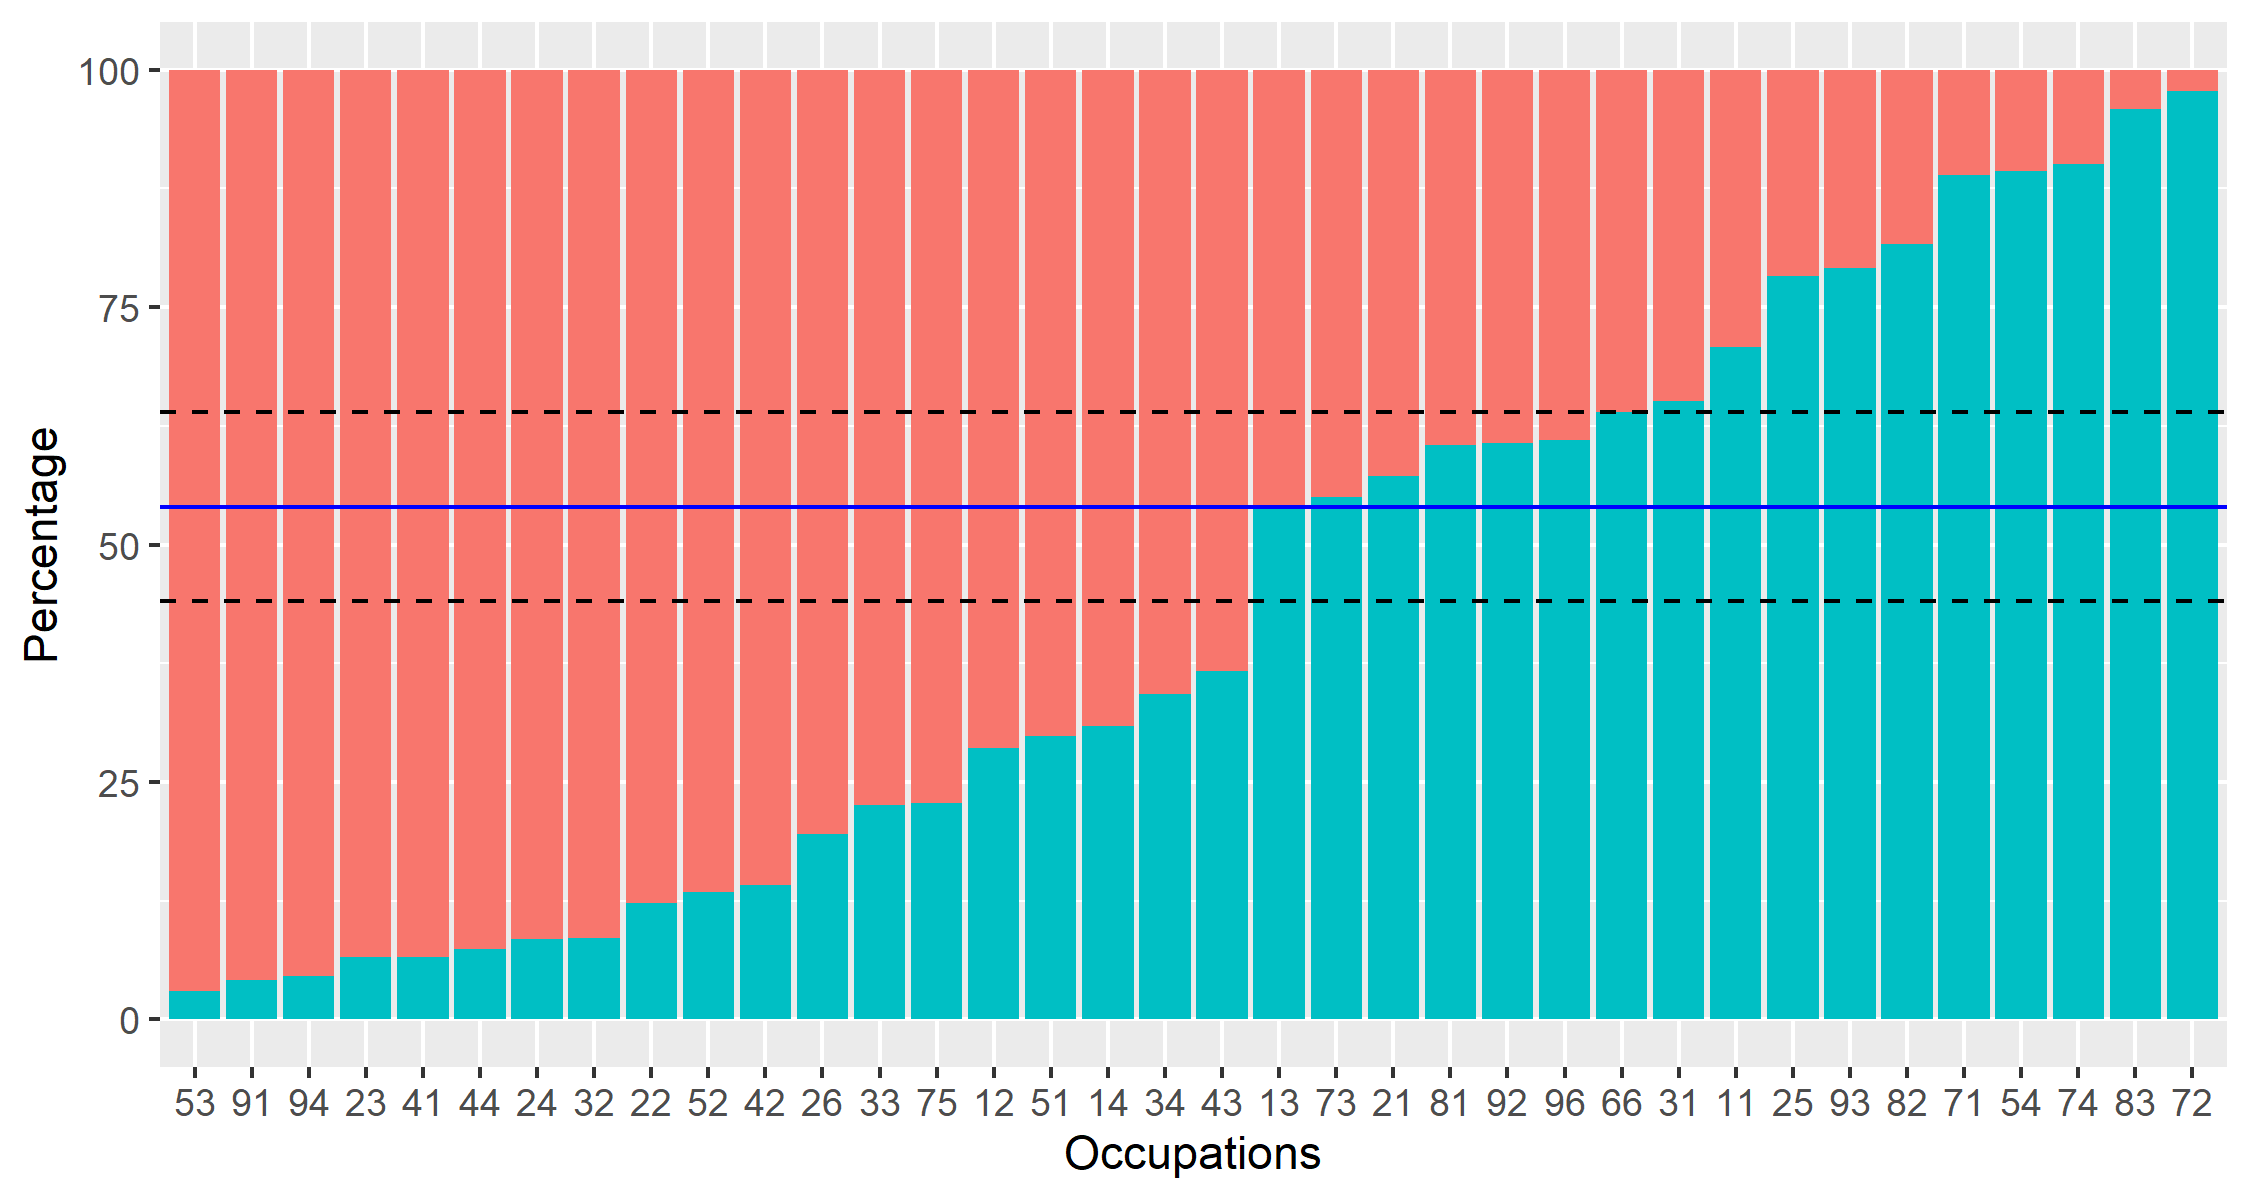
\includegraphics[width=400pt]{gen_occ18.png}
	\caption{Distribution of Employment in RLMS 2018 by Occupation and Gender}\label{fig:2.2}
\end{figure}
	
\begin{table}[htbp!]
		\centering
		\def\arraystretch{1} 
		\caption{Industries by Strength of Female Proportion, RLMS 2018}
		\label{tab:2.1}
		\begin{tabular}{p{2.5cm}l>{\raggedleft\arraybackslash}p{1.5cm}>{\raggedleft\arraybackslash}p{3cm}>{\raggedleft\arraybackslash}p{1.5cm}}
			\hline \hline
			\textbf{Category} & \textbf{Sector} & \textbf{N fem} & \textbf{\% fem} & \textbf{N total} \\ 
			\hline
			Female  & Social Services & 37 & 92.5\% &  40 \\ 
			dominated  & Other & 17 & 89.5\% &  19 \\ 
			& Education & 609 & 88.0\% & 692 \\ 
			& Public Health & 412 & 85.7\% & 481 \\ 
			& Real Estate Operations & 19 & 79.2\% &  24 \\ 
			& Government and Public Administration & 155 & 78.7\% & 197 \\ 
			& General Public Services & 15 & 75.0\% &  20 \\ 
			& Finance & 107 & 73.8\% & 145 \\ 
			& Science, Culture & 100 & 70.4\% & 142 \\ 
			& Jurisprudence & 19 & 67.9\% &  28 \\ \hline
			Neutral & Mass Media, Telecommunications & 24 & 63.2\% &  38 \\ 
			& Trade, Consumer Services & 738 & 62.8\% & 1175 \\ 
			& Light industry, Food industry & 209 & 55.0\% & 380 \\ 
			& Sports, Tourism,Entertainment & 18 & 54.5\% &  33 \\ \hline
			Male & Military Industrial Complex & 67 & 41.1\% & 163 \\ 
			dominated & Housing and Community Services & 95 & 39.1\% & 243 \\ 
			& Chemical Industry & 14 & 38.9\% &  36 \\ 
			& Civil Machine Construction & 51 & 37.8\% & 135 \\ 
			& Agriculture & 79 & 33.9\% & 233 \\ 
			& Transportation, Communication & 186 & 33.6\% & 553 \\ 
			& Information Technology & 9 & 32.1\% &  28 \\ 
			& Energy or Power Industry & 41 & 31.3\% & 131 \\ 
			& Army, Internal Security & 90 & 30.1\% & 299 \\ 
			& Other Heavy Industry & 60 & 28.7\% & 209 \\ 
			& Oil and Gas Industry & 52 & 23.5\% & 221 \\ 
			& Wood, Timber, Forestry & 7 & 21.2\% &  33 \\ 
			& Construction & 73 & 18.7\% & 391 \\ \hline
			& Total & 3303 &54.3\% & 6089 \\ \hline
		\end{tabular}
\end{table}
	
\begin{table}[!ht]
	\centering
	\caption{Occupations by Strength of Female Proportion, RLMS 2018}
	\label{tab:2.2}
		\begin{small}
			\begin{tabular}{cp{10cm}ccc}
				\hline
				& \textbf{Occupation} & \textbf{N fem} & \textbf{\% fem} & \textbf{N total} \\ 
				\hline
				1 & Personal Care Workers & 97 & 97.0\% & 100 \\ 
				2 & Cleaners and Helpers & 163 & 95.9\% & 170 \\ 
				3 & Food Preparation Assistants & 21 & 95.5\% &  22 \\ 
				4 & Teaching Professionals & 370 & 93.4\% & 396 \\ 
				5 & General and Keyboard Clerks & 71 & 93.4\% &  76 \\ 
				6 & Other Clerical Support Workers & 25 & 92.6\% &  27 \\ 
				7 & Business and Administration Professionals & 97 & 91.5\% & 106 \\ 
				8 & Health Associate Professionals & 192 & 91.4\% & 210 \\ 
				9 & Health Professionals & 79 & 87.8\% &  90 \\ 
				10 & Sales Workers & 350 & 86.6\% & 404 \\ 
				11 & Customer Services Clerks & 67 & 85.9\% &  78 \\ 
				12 & Legal, Social and Cultural Professionals & 169 & 80.5\% & 210 \\ 
				13 & Business and Administration Associate Professionals & 517 & 77.4\% & 668 \\ 
				14 & Food Processing, Woodworking, Garment and Other Craft and Related Trades Workers & 51 & 77.3\% &  66 \\ 
				15 & Administrative and Commercial Managers & 25 & 71.4\% &  35 \\ 
				16 & Personal Services Workers & 172 & 70.5\% & 244 \\ 
				17 & Hospitality, Retail and Other Services Managers & 38 & 69.1\% &  55 \\ 
				18 & Legal, Social, Cultural and Related Associate Professionals & 69 & 65.7\% & 105 \\ \hline
				19 & Numerical and Material Recording Clerks & 100 & 63.3\% & 158 \\ 
				20 & Production and Specialized Services Managers & 139 & 46.0\% & 302 \\ 
				21 & Handicraft and Printing Workers & 9 & 45.0\% &  20 \\ \hline
				22 & Science and Engineering Professionals & 101 & 42.8\% & 236 \\ 
				23 & Stationary Plant and Machine Operators & 72 & 39.6\% & 182 \\ 
				24 & Agricultural, Forestry and Fishery Laborers & 11 & 
				39.3\% &  28 \\ 
				25 & Refuse Workers and Other Elementary Workers & 30 & 39.0\% &  77 \\ 
				26 & Miscellaneous non-ISCO & 9 & 36.0\% &  25 \\ 
				27 & Science and Engineering Associate Professionals & 120 & 34.9\% & 344 \\ 
				28 & Chief Executives, Senior Officials and Legislators & 7 & 29.2\% &  24 \\ 
				29 & Information and Communications Technology Professionals & 15 & 21.7\% &  69 \\ 
				30 & Laborers in Mining, Construction, Manufacturing and 
				Transport & 24 & 20.9\% & 115 \\ 
				31 & Assemblers & 11 & 18.3\% &  60 \\ 
				32 & Building and Related Trades Workers (excluding Electricians) & 23 & 11.1\% & 207 \\ 
				33 & Protective Services Workers & 23 & 10.7\% & 215 \\ 
				34 & Electrical and Electronic Trades Workers & 16 & 9.9\% & 162 \\ 
				35 & Drivers and Mobile Plant Operators & 23 & 4.1\% & 558 \\ 
				36 & Metal, Machinery and Related Trades Workers & 6 & 2.2\% & 267 \\ 
				\hline
			\end{tabular}
		\end{small}
	\end{table}



\hspace{-1.8em} \textbf{Adaptation of Neuman and Weiss}

The Neuman and Weiss model provides an estimation of the depreciation rate 
for human capital, but by itself is unable to identify how much of that  
depreciation is external or internal. External depreciation is due to 
obsolescence (as new technologies make skills redundant) and internal 
depreciation is due to factors related to the individual. Neuman and Weiss 
had access in their empirical application to data about the technology 
level of the Israeli firms to which the workers belonged. They were able to 
show the differential effect on depreciation of workers in `high-tech 
firms', thus providing evidence in support of their model. If depreciation 
is greater for the workers in high technology industries, the amount by 
which depreciation is greater for such workers can be attributed to 
obsolescence, which is what they find. In the present paper, we do not have 
access to data about the technology level of firms, but we are able to 
exploit two variations that also help us to understand better the 
depreciation phenomenon: gender segregation is the first one of these two 
variations. Examining differences in depreciation rate by the gender 
segregation classification helps us to identify internal and external 
depreciation based on a conjecture. The conjecture is that external 
depreciation would have a greater affect by  industry sector, as 
technological change would propagate more rapidly through a sector rather 
than through occupations, which are dispersed across sectors. 

Table \ref{tab:2.3} depicts average rates of human capital loss due to 
experience and education by the female- and male-dominated industrial 
sectors and occupations. Industry or sector related differences does show 
difference in the depreciation rate, with depreciation rate being higher 
for male dominated industrial sectors. These are engineering and technology 
oriented sectors, compared to administration, services, and education which 
are the female dominated sectors. The depreciation does not appear to vary 
across occupational groupings - male dominated and female dominated 
occupation groupings have similar depreciation rates. These findings need 
to be treated as preliminary findings as they are only point estimates of 
depreciation, evaluated at mean values. 

A second adaptation of the Neuman and Weiss approach is to consider data on 
occupational routineness. In the next sub-section we follow a research path 
that was first laid out by \cite{acemoglu2011} to understand the impact of 
automation on the labor market. Following the Neuman and Weiss logic, the 
prior hypothesis would be that obsolescence will have higher effect on jobs 
with more routine tasks. To the extent that there is less of a difference 
in depreciation according to routineness measures, we can infer that there 
is less effect of obsolescence and more effect of intrinsic depreciation;  
or that obsolescence of human capital is less related to routineness and 
threat of automation. 


\begin{table}[htbp!]
	\centering 
	\caption{Average Human Capital Depreciation Rates (DR) by Female- and Male-dominated Industries and Occupations, RLMS 2018} 
	\label{tab:2.3} 
	\begin{tabular}{clcccc}
		\hline
		& \textbf{Statistic} &\textbf{Ind\_F}& \textbf{Ind\_M} & \textbf{occfemale} & \textbf{occmale} \\ 
		\hline
		1 & Experience, mean  & 23.45 & 22.97 & 21.67 & 23.48 \\ 
		2 & Education, mean & 14.06 & 13.01 & 13.67 & 12.67 \\ 
		\midrule
		3 & DR Experience, \% & 0.89 & 1.82 & 1.55 & 1.40 \\ 
		4 & DR Education, \% & 0.00 & 0.00 & 0.00 & 0.00 \\ 
		5 & DR Human Capital, \% & 0.89 & 1.82 & 1.55 & 1.40 \\ 
		\hline
	\end{tabular}
\end{table} 


\subsection{Depreciation and Occupational Routineness}

In addition to the examination of human capital depreciation rates in 
gender-dominated industries and occupations, we explore differences in 
depreciation  between groups generated by using an array of routine and 
non-routine task content metrics for jobs. This is important in light of 
discussion about computers and robots taking over routine oriented jobs. In 
this analysis, we rely on a recent literature of job classification based 
on task intensity measures  \citet{Mihaylov_2019}. These measures are based 
on the textual analysis of description of jobs in the ISCO 08 
classification. Each job lists a detailed set of activities or tasks 
performed as part of the job, and these activities are rated according to 
whether they are vulnerable to automation in which case they are classified 
as Routine (R), otherwise they are Non-Routine (NR). Tasks are also 
classified depending on their Cognitive (C) or Manual (M) requirements; 
Cognitive tasks are further classified as mainly Analytic (A) or 
Interactive (I). The results is a five-fold classification of tasks, which 
is subsequently used to develop a set of measures depending on the 
incidence of these tasks in the job description.

For purpose of this analysis, we use two of these measures. Routine Task 
Intensity measure (RTI) denotes a score difference between the summed 
routine task indices and the summed non-routine task indices: $(RC + RM) - 
(NRA + NRI + NRM)$ - it is a net measure of job routineness or 
vulnerability to automation. We also use a gross measure that brings 
together the non-routine task indices: $NRA + NRI + NRM$. Using the k-means 
clustering technique for the metrics described, we created two respective 
categorical variables (drti and dnraim) with categories capturing 
\textit{high, medium,} and \textit{low} manifestations of the features.

Table \ref{tab:2.4} shows the results of comparing depreciation rates between individuals whose jobs invoke routine or non-routine tasks at a high, medium, or low level. The findings suggest that depreciation explained by experience does not differ substantially between people with jobs with varying routine task intensity. The same outcome also applies to workers varying in the degree of non-routine content at their jobs. As with the findings regarding gender, these should be regarded as preliminary findings subject to further analysis. However, it does appear that the automation aspect of technological change may not be affecting the rate of depreciation of skills - both routine and non-routine intensive jobs undergo depreciation, though it is possibly that the underlying causal factors may be different. 

\begin{table}[htbp!]
	\centering
	\caption{Average Human Capital Depreciation Rates (DR) by Routineness Classification, RLMS 2018}
	\label{tab:2.4}
	\begin{tabular}{clccc|cccccc}
		\hline
		& \textbf{Statistic} & \textbf{High} & \textbf{Low} & \textbf{Medium} & \textbf{High} & \textbf{Low} & \textbf{Medium} \\ 
		\hline
& & \multicolumn{3}{c|}{Net Routine Task Intensity} & \multicolumn{3}{c} {Gross Non-Routiness Measure} \\
		\hline
		1 & Measure & drti & drti & drti & dnraim & dnraim & dnraim \\ 
		2 & Experience, mean  & 21.44 & 22.79 & 22.76 & 22.94 & 22.22 & 22.05 \\ 
		3 & Education, mean & 12.86 & 13.67 & 12.8 & 13.66 & 12.76 & 13.02 \\ 
		\hline
		4 & DR Experience, \% & 1.8 & 1.5 & 1.64 & 1.62 & 1.73 & 1.48 \\ 
		5 & DR Education, \% & 0 & 0 & 0 & 0 & 0 & 0 \\ 
		6 & DR Human Capital, \% & 1.8 & 1.5 & 1.64 & 1.62 & 1.73 & 1.48 \\ 
		\hline
	\end{tabular}
\end{table}

\section{Summarized Findings and Policy Conclusions}


\subsection{Summarized Findings}

This paper has covered substantive technical material. The main finding are 
summarized in the points below:- 


\begin{itemize}

\item \textbf{Depreciation of 2\%} The topic of depreciation of 
human capital is important from the policy perspective because increasing 
the human capital can be made both by the creation of human capital as well 
as reducing the depreciation of human capital to the extent possible. In 
this paper per first presented an overview of the literature regarding 
depreciation of human capital and present estimates of depreciation in the 
Russian Federation. Depreciation appears to be around 2\% per year in the 
most recent finding, with the depreciation mostly attributed to 
depreciation of human capital acquired with experience (Table\ref{tab:1.2}).


\item \textbf{Depreciation declining then increasing}  The 
pattern of the depreciation rate indicates a gentle decline followed by an 
increase in the period 1994-2018 (Table \ref{tab:1.2} and Table 
\ref{tab:1.3}). This pattern is a reflection of the inverted-U shaped 
pattern of the rates of return to education. It is possible that 
depreciation may be an explanation for the observed tendency in the returns 
to education.


\item  \textbf{University educated individuals make more 
post-school investment too} In estimating rates of depreciation, we 
undertake an exploration of a related parameter that represents 
post-schooling investment in human capital. The data indicates that 
post-schooling investment for those with vocational education is 
indistinguishable from those with only secondary education. However, those 
with university education appear to be investing more in their working 
period (Table \ref{tab:1.4}).


\item  \textbf{Males may be experiencing higher depreciation 
than 
females} 
The paper explored differences in depreciation rates across industrial and 
occupation groupings denoted by levels of gender segregation Depreciation 
rates appear to be higher in male dominated industrial sectors but gender 
related occupational groupings do not show this differential. The evidence 
suggests that external depreciation due to obsolescence may be a dominant 
component of the depreciation of human capital (Table \ref{tab:2.3}). 


\item \textbf{Automation possibilities of jobs may not be 
related 
to depreciation} The paper used a relatively recent classification of jobs 
regarding the potential for automation depending on the routine or 
non-routine nature of tasks. It was hypothesized that routine intensive 
jobs which are more likely to be taken overy by computers may suffer from a 
higher depreciation rate, but the data do not reveal differences in 
depreciation rate by routine task intensity (Table \ref{tab:2.4}).

\end{itemize}


\subsection{Policy Conclusions}

These findings and the context of the larger literature on depreciation and 
the returns to education results in the following policy conclusions:

\begin{itemize}

\item  \textbf{Emphasize lifelong learning to augment human 
capital 
wealth} Non-cognitive skills that are 
formed throughout the lifetime have equally strong effects on productivity  
\parencite{kautz2014}. Research in Norway backs up this claim 
\parencite{midtsundstad2019}. Investment in lifelong learning will be more 
relevant for the Russian Federation as the average age of retirement moves 
out \parencite{kilpi2012, paccagnella2016}.
 

\item \textbf{Renovate curriculum and stress extra-curricular education at 
all levels to emphasize 
learning to learn} Enhanced lifelong learning capacity begins at an early 
age \parencite{kautz2014}. Curriculum from early grades to university will 
benefit from greater emphasis on application of critical thinking and 
problem solving skills. Extra-curricular education is geared towards 
non-cognitive skills and the Russian Federation is already a world leader 
in this area. 

\item  \textbf{Support internal migration which brings better efficiency 
and equity to the labor market} The Russian Federation benefits from 
substantive internal migration and migration from the former Soviet 
republics that are now independent \parencite{tarasyev2018}. Policies 
should support this migration by easing restrictions on worker movements 
\parencite{oshchepkov2015}. 

\item \textbf{Investigate more closely the determinants and the impact of 
depreciation of human capital in the Russian context} There are a number of 
areas where further inquiry will provide useful insights. In addition to 
the areas already mentioned above of migration, curriculum and life-long 
learning programs, the following research areas are promising: (i) How 
returns to education over the lifetime vary for STEM disciplines 
\parencite{deming2018}; (ii) How digitization of jobs in relation to 
automation may or may be related to the findings regarding routineness 
\parencite{evangelista2014,cirillo2019}; (iii) How is aging related to 
changes in productivity and what are effective programs to counter the 
effect of aging, such as deployment of specific equipment and 
infrastructure for older people and the formation of mixed-age work teams 
\parencite{gobel2009,gobel2013}.


\printbibliography

\newpage
\section*{Appendix}
\addcontentsline{toc}{section}{Appendix}%

\setcounter{table}{0}
\renewcommand{\thetable}{A\arabic{table}}

\setcounter{figure}{0}
\renewcommand{\thefigure}{A\arabic{figure}}

\begin{center}
	\begin{figure}[htbp!]
\begin{minipage}[b]{1\linewidth}
			\centering
			%\hspace*{-0.7in}
			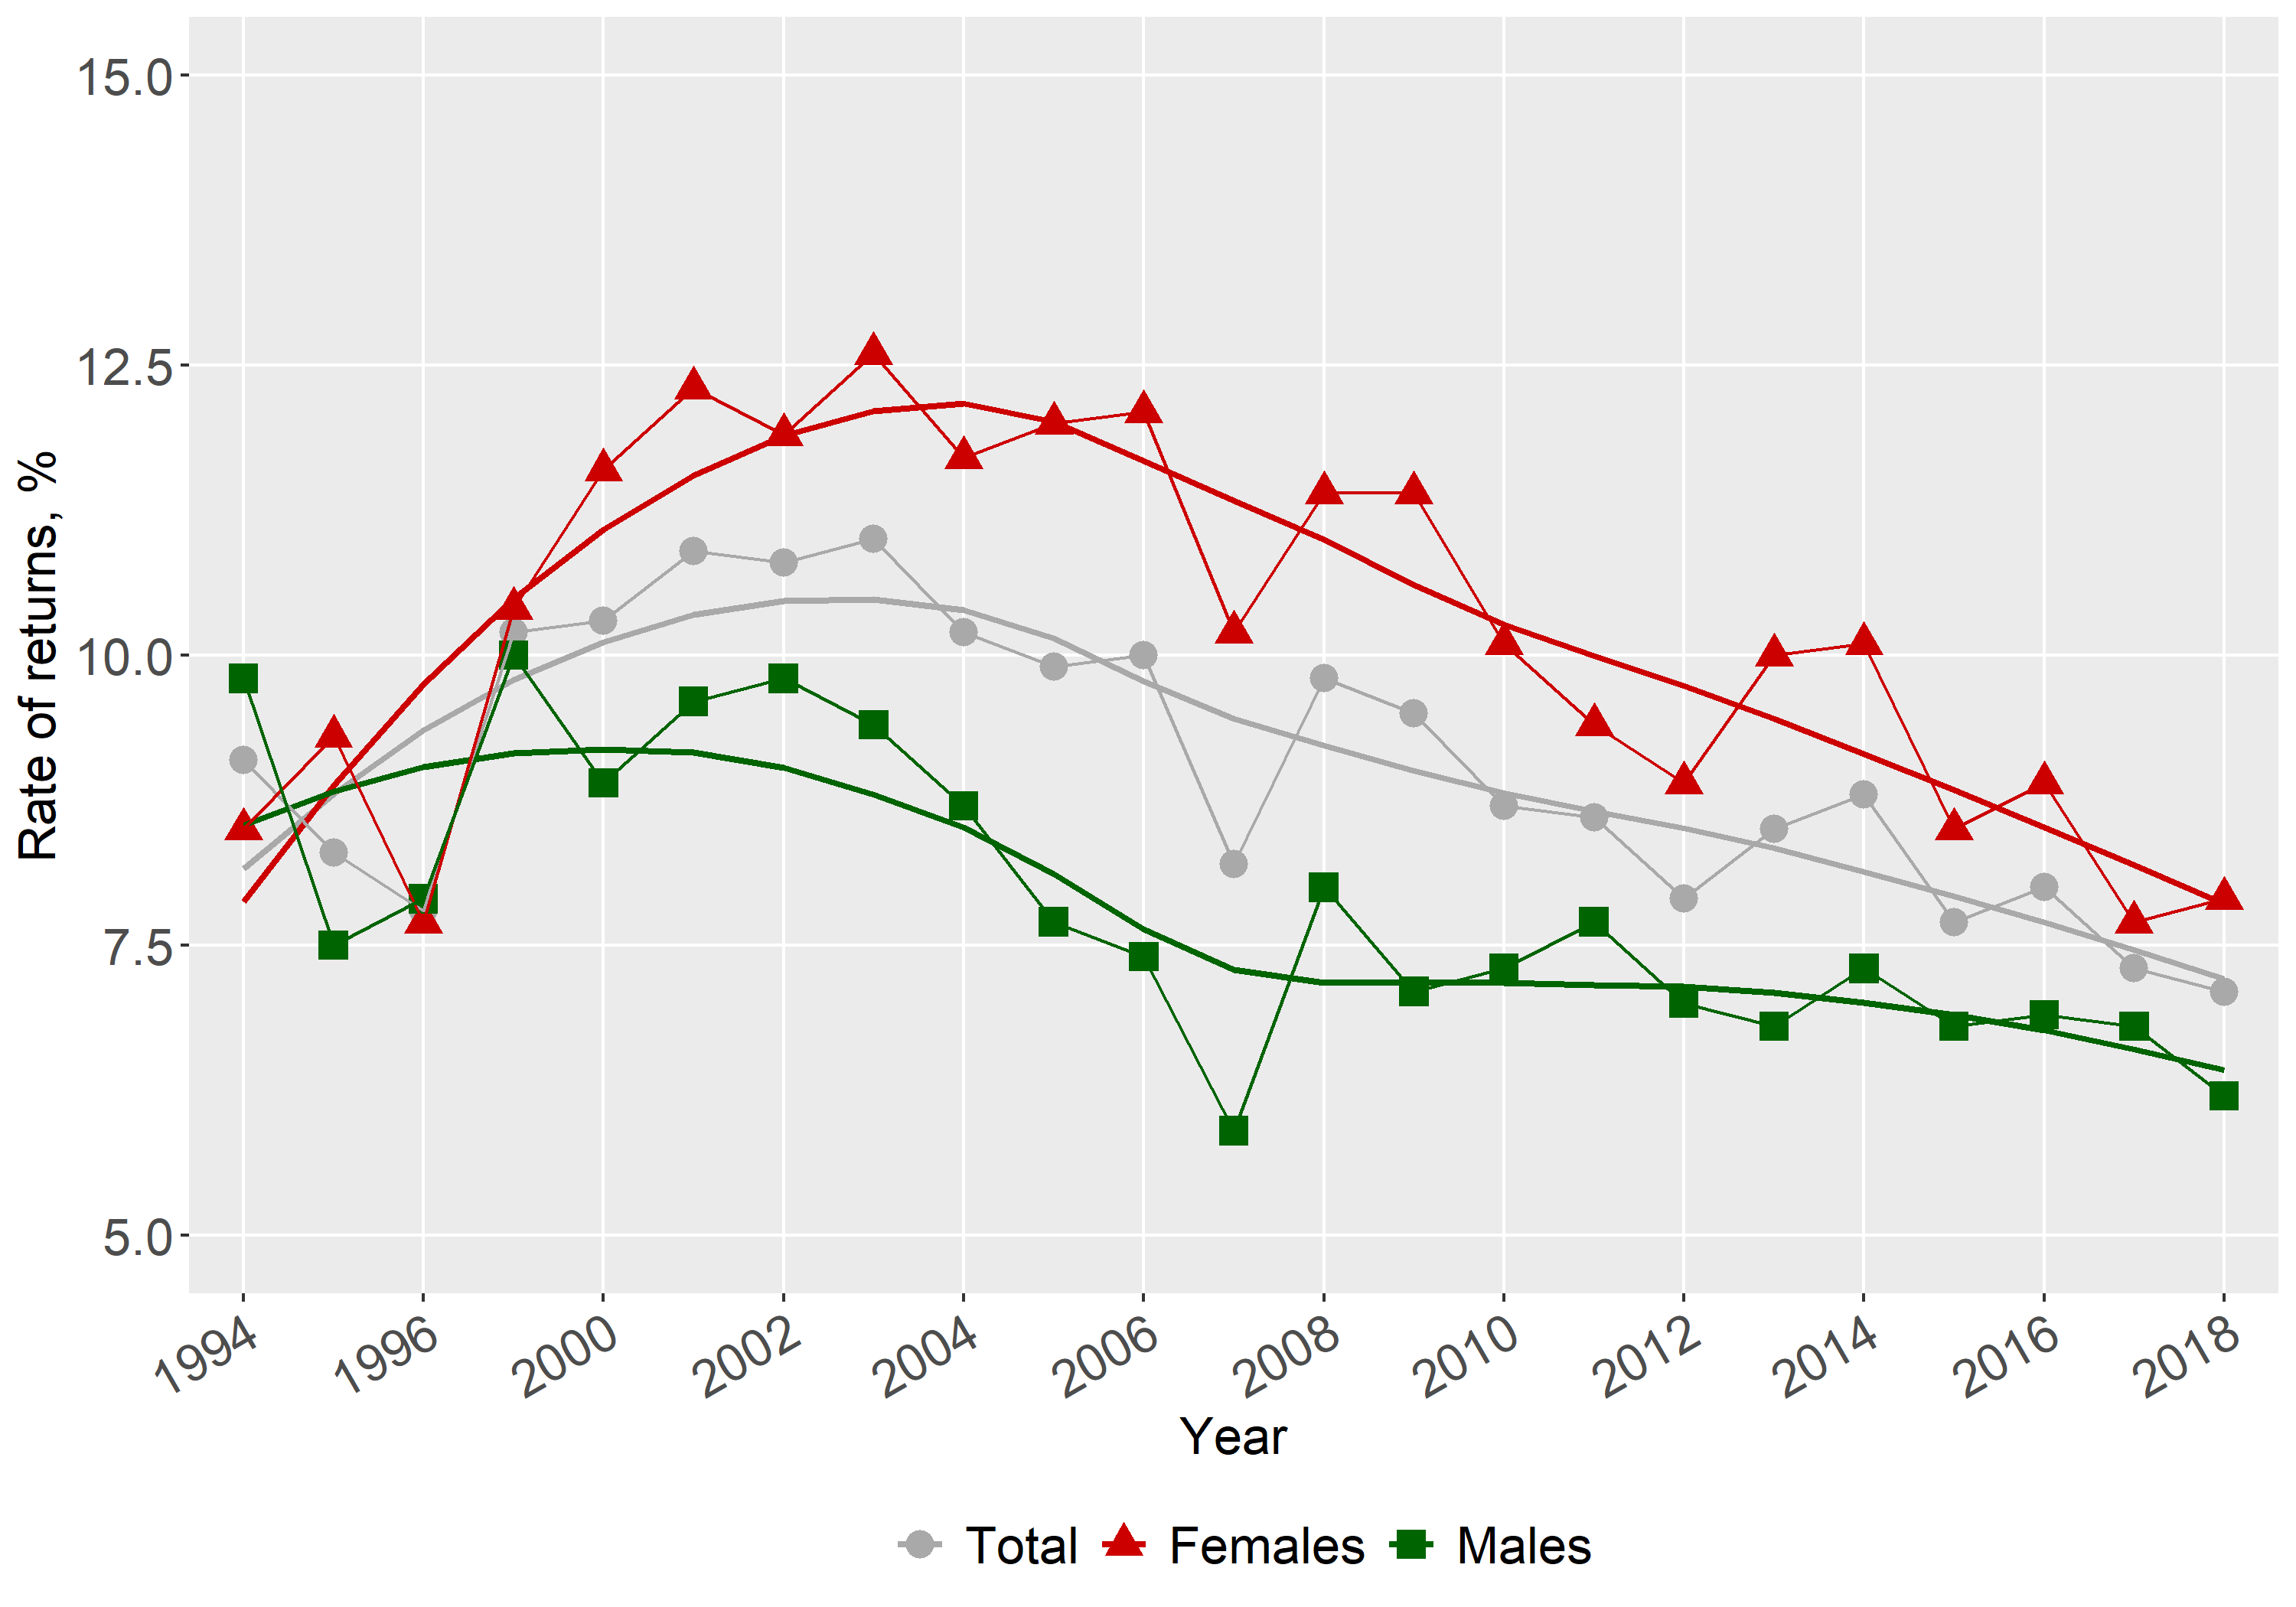
\includegraphics[width=6in]{re_edu.png}
			% plot 1
		\end{minipage}
			\caption{Mincerian Rates of Return to Education in Russia 1994 to 2018}\label{fig:7.6}
	\end{figure}
\end{center}


\end{document}
